%%%% main.tex, 2022/08/10, 2.5
%%%% Copyright (C) 2020 Vinicius Pegorini (vinicius@utfpr.edu.br)
%%
%% This work may be distributed and/or modified under the conditions of the
%% LaTeX Project Public License, either version 1.3 of this license or (at your
%% option) any later version.
%% The latest version of this license is in
%%   http://www.latex-project.org/lppl.txt
%% and version 1.3 or later is part of all distributions of LaTeX version
%% 2005/12/01 or later.
%%
%% This work has the LPPL maintenance status `maintained'.
%%
%% The Current Maintainer of this work is Vinicius Pegorini.
%%
%% This work consists of the files utfprpb.cls, utfprpb.tex, and
%% utfprpb-dados.tex.
%%
%% The Current Maintainer of this work is Vinicius Pegorini.
%% Updated by:
%% - Marco Aurélio Graciotto Silva;
%% - Rogério Aparecido Gonçalves;
%% - Luiz Arthur Feitosa dos Santos.
%%
%% This work consists of the files utfpr.cls, main.tex, and
%% variaveis.tex.
%% A brief description of this work is in readme.md.

%% ####################################################
%%
%% >> Atenção - Leia isso antes de usar esse template<< 
%%
%% Esse template foi desenvolvido por professores,  com a intenção de ajudar os alunos com as entregas na biblioteca. Não há uma equipe especializada e dedicada mantendo tal template, mas sim professores trabalhando além das suas funções básicas, que são: ensino, pesquisa e extensão.
%
%% Também os mantenedores deste template não são especializados em LaTeX, muito menos em normas da ABNT. Todos que contribuíram com o template fizeram isso visando deixá-lo o mais próximo possível das normas da ABNT e das regras, anseios e expectativas da biblioteca da UTFPR. É muito importante entender que os desenvolvedores do template não têm relação direta com a biblioteca ou com a ABNT. Ou seja, não são os desenvolvedores do template que ditam as regras e normas dos textos que devem ser entregues à biblioteca.

%%É válido informar também, que como não há uma equipe dedicada e especializada, o tempo para colaborar com o template é curto. Desta forma, pode ser que não sejam empregadas as melhores técnicas, métodos e ferramentas para o desenvolvimento do template. Também pode acontecer do template não atender completamente todos os anseios e exigências da ABNT e da biblioteca, pois por exemplo, muitas regras de redação possuem questões interpretativas. Assim, o template sempre estará em contínua evolução e seria extremamente interessante que as pessoas (alunos,  professores,  técnicos e entusiastas) colaborarem com a evolução do template. Toda ajuda será bem vinda! Isso pode ser feito enviando e-mail para os desenvolvedores, desta forma, assim que possível esses vão tentar melhorar o template.

%%O template é apenas mais uma ferramenta para o desenvolvimento de trabalhos para a biblioteca. Todavia, podem existir outros templates LaTeX. Assim como há templates em outros formatos, que não o LaTeX. O mais importante é que qualquer pessoa, utilizando a princípio qualquer ferramenta, pode desenvolver textos que atendem os requisitos da biblioteca apenas estudando, interpretando e seguindo as regras da UTFPR e da ABNT, que estão disponíveis na página Web da instituição. O template é só um facilitador.

%%Por fim,  é necessário entender que infelizmente o ambiente LaTeX pode ser complexo e gerar resultados distintos dependendo do: sistema operacional,  pacotes LaTeX utilizados,  configurações alteradas, editor utilizado, a forma que está sendo redigida textos, figuras,  etc. Assim não há como garantir que o resultado final será o esperado.  Dito tudo isso,  >>UTILIZE ESSE TEMPLATE POR SUA CONTA E RISCO<<. Os desenvolvedores e colaboradores deste template não se responsabilizam pelo resultado do uso deste template e se eximem de qualquer responsabilidade.

%###################################################


% Prévia do TCC2. Compilar este arquivo a partir da pasta docs/report.
\PassOptionsToPackage{pdfa}{hyperref}
\documentclass[
  12pt,a4paper,oneside,openright,
  sumario=abnt-6027-2012,chapter=TITLE,
  pretextualoneside,fontetimes,semrecuonosumario,pardeassinaturas,
  english,brazil
]{utfpr}

% Compatibilidade do pdfx com XeTeX/Tectonic.
\ifdefined\XeTeXversion
  \ifdefined\pdfcreationdate\else
    \let\pdfcreationdate\creationdate
  \fi
\fi
\usepackage[a-3b,mathxmp]{pdfx}[2018/12/22]
%%%% configuracoes.tex, 2022/05/02, 2.4a

%% ####################################################
%%
%% >> Atenção - Leia isso antes de usar esse template<< 
%%
%% Esse template foi desenvolvido por professores,  com a intenção de ajudar os alunos com as entregas na biblioteca. Não há uma equipe especializada e dedicada mantendo tal template, mas sim professores trabalhando além das suas funções básicas, que são: ensino, pesquisa e extensão.
%
%% Também os mantenedores deste template não são especializados em LaTeX, muito menos em normas da ABNT. Todos que contribuíram com o template fizeram isso visando deixá-lo o mais próximo possível das normas da ABNT e das regras, anseios e expectativas da biblioteca da UTFPR. É muito importante entender que os desenvolvedores do template não têm relação direta com a biblioteca ou com a ABNT. Ou seja, não são os desenvolvedores do template que ditam as regras e normas dos textos que devem ser entregues à biblioteca.

%%É válido informar também, que como não há uma equipe dedicada e especializada, o tempo para colaborar com o template é curto. Desta forma, pode ser que não sejam empregadas as melhores técnicas, métodos e ferramentas para o desenvolvimento do template. Também pode acontecer do template não atender completamente todos os anseios e exigências da ABNT e da biblioteca, pois por exemplo, muitas regras de redação possuem questões interpretativas. Assim, o template sempre estará em contínua evolução e seria extremamente interessante que as pessoas (alunos,  professores,  técnicos e entusiastas) colaborarem com a evolução do template. Toda ajuda será bem vinda! Isso pode ser feito enviando e-mail para os desenvolvedores, desta forma, assim que possível esses vão tentar melhorar o template.

%%O template é apenas mais uma ferramenta para o desenvolvimento de trabalhos para a biblioteca. Todavia, podem existir outros templates LaTeX. Assim como há templates em outros formatos, que não o LaTeX. O mais importante é que qualquer pessoa, utilizando a princípio qualquer ferramenta, pode desenvolver textos que atendem os requisitos da biblioteca apenas estudando, interpretando e seguindo as regras da UTFPR e da ABNT, que estão disponíveis na página Web da instituição. O template é só um facilitador.

%%Por fim,  é necessário entender que infelizmente o ambiente LaTeX pode ser complexo e gerar resultados distintos dependendo do: sistema operacional,  pacotes LaTeX utilizados,  configurações alteradas, editor utilizado, a forma que está sendo redigida textos, figuras,  etc. Assim não há como garantir que o resultado final será o esperado.  Dito tudo isso,  >>UTILIZE ESSE TEMPLATE POR SUA CONTA E RISCO<<. Os desenvolvedores e colaboradores deste template não se responsabilizam pelo resultado do uso deste template e se eximem de qualquer responsabilidade.

%###################################################

%% Pacotes carregados nas classes:
%%   memoir: abstract, appendix, array, booktabs, ccaption, chngcntr, chngpage, dcolumn, delarray, enumerate, epigraph, framed,
%%           ifmtarg, ifpdf, index, makeidx, moreverb, needspace, newfile, nextpage, parskip, patchcmd, setspace, shortvrb, showidx,
%%           tabularx, titleref, titling, tocbibind, tocloft, verbatim, verse.
%%   memoir (similares): crop, fancyhdr, geometry, sidecap, subfigure, titlesec.
%%   abntex2: babel, bookmark, calc, enumitem, ifthen, hyperref, textcase.
%%   utfprpgtex: abntex2cite, ae, algorithmic, amsmath, backref, breakurl, caption, cmap, color, eepic, epic, epsfig, etoolbox,
%%               fancyhdr, fix-cm, fontenc, glossaries, graphics, graphicx, helvet, hyphenat, indentfirst, inputenc, lastpage,
%%               morewrites, nomencl, sfmath, sistyle, substr, times, xtab.


%% Pacotes adicionais (\usepackage[options]{package})
\usepackage{bigdelim, booktabs, colortbl, longtable, multirow}%% Ferramentas para tabelas
\usepackage{amssymb, amstext, amsthm, icomma}%% Ferramentas para linguagem matemática
\usepackage{pifont, textcomp, wasysym}%% Símbolos de texto
\usepackage{lipsum}				% para geração de dummy text
\usepackage{subfig}             % para adicionar figuras lado a lado no texto                    
\usepackage{pdfpages}           % para adicionar documentos pdf ao trabalho
\usepackage{xspace}


% luiz: primeira letra maiúscula
% solução 1
%\usepackage{stringstrings}
%\newcommand{\firstcap}[1]{\caselower[e]{#1}\capitalize{\thestring}}

% solução 2 - não usei essa
% \usepackage[utf8]{inputenc}
% \usepackage{datatool-base}
% \usepackage{mfirstuc}

% Formatação do título da seção - primeira letra caixa alta e o resto em caixa baixa.
% \usepackage[explicit]{titlesec}
% \usepackage{lipsum}
% \titleformat{\section}{\normalfont}{\thesection}{1em}{\textbf{\firstcap{#1}}} % funciona mas apenas para o título da seção e não para o sumário (a configuração do sumário está mais para baixo

% luiz: define o underline colorido.
% https://github.com/abntex/abntex2-contrib/blob/master/customizacoes/pucminas/abntex2-pucminas.sty
% acabei não usando o black e o coloruline da solução do link

\usepackage[normalem]{ulem} % para o underline colorido na seção quaternária
\renewcommand*{\cftsubsubsectionfont}{\normalfont\uline} % underline no sumário
\setsubsubsecheadstyle{\ABNTEXsubsubsectionfont\ABNTEXsubsubsectionfontsize\ABNTEXsubsubsectionupperifneeded\uline} %underline no título da subsubsection

% luiz: bibliografia - opções

%% Comandos personalizados (\newcommand{name}[num]{definition})
\newcommand{\cpp}{\texttt{C$++$}}%% C++
\newcommand{\latex}{\LaTeX\xspace}%% LaTeX
\newcommand{\ds}{\displaystyle}%% Tamanho normal das equações
\newcommand{\bsym}[1]{\boldsymbol{#1}}%% Texto no modo matemático em negrito
\newcommand{\mr}[1]{\mathrm{#1}}%% Texto no modo matemático normal (não itálico)
\newcommand{\der}{\mr{d}}%% Operador diferencial
\newcommand{\deri}[2]{\frac{\der #1}{\der #2}}%% Derivada ordinária
\newcommand{\derip}[2]{\frac{\partial #1}{\partial #2}}%% Derivada parcial
\newcommand{\pare}[1]{\left( #1 \right)}%% Parênteses
\newcommand{\colc}[1]{\left[ #1 \right]}%% Colchetes
\newcommand{\chav}[1]{\left\lbrace #1 \right\rbrace}%% Chaves
\newcommand{\sen}{\operatorname{sen}}%% Operador seno
\newcommand{\senh}{\operatorname{senh}}%% Operador seno hiperbólico
\newcommand{\tg}{\operatorname{tg}}%% Operador tangente
\newcommand{\tgh}{\operatorname{tgh}}%% Operador tangente hiperbólico
\newcommand{\seqref}[1]{Equação~\eqref{#1}}%% Referência de uma única equação
\newcommand{\meqref}[1]{Equações~\eqref{#1}}%% Referência de múltiplas equações
\newcommand{\citep}[1]{\cite{#1}}%% Atalho para citação implícita
\newcommand{\citet}[1]{\citeonline{#1}}%% Atalho para citação explícita
\newcommand{\citepa}[1]{(\citeauthor{#1})}%% Atalho para citação implícita (somente autor)
\newcommand{\citeta}[1]{\citeauthoronline{#1}}%% Atalho para citação explícita (somente autor)
\newcommand{\citepy}[1]{(\citeyear{#1})}%% Atalho para citação implícita (somente ano)
\newcommand{\citety}[1]{\citeyear{#1}}%% Atalho para citação explícita (somente ano)

\newcommand{\fonteTexto}[1]{\renewcommand{\familydefault}{#1}}

% Define o caminho das figuras
\graphicspath{{figuras/}}

% Define a fonte ara helvet que é uma fonte similar à Arial, se for usar a Arial tem que mudar o compilador para XeLaTex, mas ai tem que arrumar os erros: https://latex.org/forum/viewtopic.php?t=25998
%\usepackage{helvet}
%\renewcommand{\familydefault}{\sfdefault}
%\usepackage{times} % para fonte time new roman
%\usepackage{pslatex} % ou essa aqui...

%\usepackage{titlesec}

%% Configuração de glossário
% \usepackage[portuguese]{nomencl}
% \usepackage[nogroupskip,nonumberlist,nopostdot,nohypertypes={acronym}]{glossaries}
% \makenoidxglossaries
\usepackage{glossaries}
\makeglossaries

% para siglas em português
\newcommand{\siglaPt}[2]
{
 \newglossaryentry{#1}{
  name=#1,
  description={#2},
  first={#2 (#1)},
  long={#2}
 }  
}

% para siglas de língua estrangeira, nessas a descrição longa fica em itálico.
\newcommand{\siglaIt}[2]
{
 \newglossaryentry{#1}{
  name=#1,
  description={\textit{#2}},
  first={\textit{#2} ({#1})},
  long={\textit{#2}}
 }  
}

%% luiz - para fazer os avisos
\usepackage{tcolorbox}

% use para criar caixas de avisos, pode ser utilizado para fazer anotações de tarefas indicadas pelo orientador/banca.
% \caixa{Atenção}{texto...}
\newcommand{\caixa}[2]{
\begin{tcolorbox}[colback=red!5!white,colframe=red!45!white, title = #1, fonttitle=\bfseries]
#2
\end{tcolorbox}
}

% Luiz - Linhas órfãs e viúvas
\widowpenalty=10000
\clubpenalty=10000

% Luiz - Caption do tamanho da Tabela
%\usepackage[width=1\textwidth]{caption}

% Luiz - configurar a margem dos itens
\setlength{\leftmargini}{1.5cm}
\setlength{\leftmarginii}{1.5cm}

%%%% variaveis.tex, 2022/05/02, 2.4a
%%%% Copyright (C) 2020 Vinicius Pegorini (vinicius@utfpr.edu.br)
%%
%% This work may be distributed and/or modified under the conditions of the
%% LaTeX Project Public License, either version 1.3 of this license or (at your
%% option) any later version.
%% The latest version of this license is in
%%   http://www.latex-project.org/lppl.txt
%% and version 1.3 or later is part of all distributions of LaTeX version
%% 2005/12/01 or later.
%%
%% This work has the LPPL maintenance status `maintained'.
%%
%% The Current Maintainer of this work is Vinicius Pegorini.
%% Updated by:
%% - Marco Aurélio Graciotto Silva;
%% - Rogério Aparecido Gonçalves;
%% - Luiz Arthur Feitosa dos Santos.
%%
%% This work consists of the files utfpr.cls, main.tex, and
%% variaveis.tex.
%%
%% A brief description of this work is in readme.txt.

%% ####################################################
%%
%% >> Atenção - Leia isso antes de usar esse template<< 
%%
%% Esse template foi desenvolvido por professores,  com a intenção de ajudar os alunos com as entregas na biblioteca. Não há uma equipe especializada e dedicada mantendo tal template, mas sim professores trabalhando além das suas funções básicas, que são: ensino, pesquisa e extensão.
%
%% Também os mantenedores deste template não são especializados em LaTeX, muito menos em normas da ABNT. Todos que contribuíram com o template fizeram isso visando deixá-lo o mais próximo possível das normas da ABNT e das regras, anseios e expectativas da biblioteca da UTFPR. É muito importante entender que os desenvolvedores do template não têm relação direta com a biblioteca ou com a ABNT. Ou seja, não são os desenvolvedores do template que ditam as regras e normas dos textos que devem ser entregues à biblioteca.

%%É válido informar também, que como não há uma equipe dedicada e especializada, o tempo para colaborar com o template é curto. Desta forma, pode ser que não sejam empregadas as melhores técnicas, métodos e ferramentas para o desenvolvimento do template. Também pode acontecer do template não atender completamente todos os anseios e exigências da ABNT e da biblioteca, pois por exemplo, muitas regras de redação possuem questões interpretativas. Assim, o template sempre estará em contínua evolução e seria extremamente interessante que as pessoas (alunos,  professores,  técnicos e entusiastas) colaborarem com a evolução do template. Toda ajuda será bem vinda! Isso pode ser feito enviando e-mail para os desenvolvedores, desta forma, assim que possível esses vão tentar melhorar o template.

%%O template é apenas mais uma ferramenta para o desenvolvimento de trabalhos para a biblioteca. Todavia, podem existir outros templates LaTeX. Assim como há templates em outros formatos, que não o LaTeX. O mais importante é que qualquer pessoa, utilizando a princípio qualquer ferramenta, pode desenvolver textos que atendem os requisitos da biblioteca apenas estudando, interpretando e seguindo as regras da UTFPR e da ABNT, que estão disponíveis na página Web da instituição. O template é só um facilitador.

%%Por fim,  é necessário entender que infelizmente o ambiente LaTeX pode ser complexo e gerar resultados distintos dependendo do: sistema operacional,  pacotes LaTeX utilizados,  configurações alteradas, editor utilizado, a forma que está sendo redigida textos, figuras,  etc. Assim não há como garantir que o resultado final será o esperado.  Dito tudo isso,  >>UTILIZE ESSE TEMPLATE POR SUA CONTA E RISCO<<. Os desenvolvedores e colaboradores deste template não se responsabilizam pelo resultado do uso deste template e se eximem de qualquer responsabilidade.

%###################################################

%% Documento
%% Luiz: Define a fonte do texto da monografia
\fonteTexto{\sfdefault} % utilize \rmdefault para Times New Roman ou \sfdefault para Arial
\TipoDeDocumento{Trabalho de Conclusão de Curso de Graduação}%% Tipo de documento: "Tese", "Dissertação" ou "Trabalho de Conclusão de Curso de Graduação", "Estágio Supervisionado"
\NivelDeFormacao{Bacharelado}%% Nível de formação: "Doutorado", "Mestrado", "Bacharelado" ou "Tecnólogo" - ATENÇÃO, isso será utilizado para alterar a formatação do trabalho, pois pode haver formatações distintas dependendo o nível/tipo de trabalho.


%% luiz
% Template LaTex criado pelo Departamento Acadêmico de Computação (DACOM)
% da Universidade Tecnológica Federal do Paraná - Campus Campo Mourão (UTFPR-CM)
% Criado e alterado pelos professores:
% - Marco Aurélio Graciotto Silva
% - Rogério Aparecido Gonçalvez
% - Luiz Arthur Feitosa dos Santos
% Esse template utiliza a licença CC BY:
% Esta licença permite que outros distribuam, remixem, adaptem e criem a partir deste trabalho, mesmo para fins comerciais, desde que atribuam o devido crédito pela criação original.
% https://creativecommons.org/licenses/by/4.0/deed.pt_BR

% Dados do curso. Caso seja BCC:
\program{Curso de Bacharelado em Ciência da Computação}
\programen{Undergraduate Program in Computer Science}
\degree{Bacharel}
\degreearea{Ciência da Computação}
% Caso seja TSI:
% \program{Curso Superior de Tecnologia em Sistemas para Internet}
% \programen{Undergradute Program in Tecnology for Internet Systems}
% \degree{Tecnólogo}
% \degreearea{Tecnologia em Sistemas para Internet}


% Dados da disciplina. Escolha uma das opções e a descomente:
% TCC1:
%\goal{Proposta de Trabalho de Conclusão de Curso de Graduação}
%\course{Trabalho de Conclusão de Curso 1}
% TCC2:
 \goal{Trabalho de Conclusão de Curso de Graduação}
 \course{Trabalho de Conclusão de Curso 2}


% Dados do TCC (precisa alterar)
\author{Alan Lima Marques}  % Seu nome
\authorbib{Marques, Alan Lima} % Seu nome para referência bibliográfica (Sobrenome, Nome)
\title{Desenvolvimento de um jogo 3D multijogador de tiro em primeira pessoa} % Título do trabalho
\titleen{Development of a 3D Multiplayer First-Person Shooter Game} % Título traduzido para inglês
\advisor{Prof. Dr. Marcos Silvano Orita Almeida} % Nome do orientador. Lembre-se de prefixar com "Prof. Dr.", "Profª. Drª.", "Prof. Me." ou "Profª. Me."}
% Se não houver corientador, comente a linha a baixo
%coadvisor{Nome Orientador completo e título} % Nome do coorientador, caso exista. Caso não exista, comente a linha.
\depositshortdate{2026} % Ano em que depositou este documento
\approvaldate{a definir} % Atualizar após a confirmação da defesa do TCC2.

% Dados do curso que não precisam de alteração
\university{Universidade Tecnológica Federal do Paraná}
\universityen{Federal University of Technology -- Paraná}
\universitycampus{Campus Campo Mourão}
\universityunit{Departamento Acadêmico de Computação}
\address{Campo Mourão, PR, Brasil}
\addressen{Campo Mourão, PR, Brazil}
\documenttype{Monografia}
\documenttypeen{Monograph}
\degreetype{Graduação}

% Banca do TCC1, preservada apenas para consulta:
% \evalboardmember{Marcos Silvano Orita Almeida}{Prof. Dr.}{Universidade Tecnológica Federal do Paraná}

% Banca do TCC1, preservada apenas para consulta:
% \evalboardmember{Alane Marie de Lima}{Profa. Dra.}{Universidade Tecnológica Federal do Paraná}

% Banca do TCC1, preservada apenas para consulta:
% \evalboardmember{Juliano Henrique Foleis}{Prof. Dr.}{Universidade Tecnológica Federal do Paraná}

%\evalboardmember{Nome completo e por extenso do Membro 2}{Título (especialização, mestrado, doutorado}{Nome completo e por extenso da instituição a qual possui vínculo}

% Banca do TCC2.
\evalboardmember{Marcos Silvano Orita Almeida}{Prof. Dr.}{Universidade Tecnológica Federal do Paraná}
\evalboardmember{Rodrigo Hübner}{Prof. Dr.}{Universidade Tecnológica Federal do Paraná}
\evalboardmember{Juliano Henrique Foleis}{Prof. Dr.}{Universidade Tecnológica Federal do Paraná}

%% Palavras-chave e keywords
%% ATENÇÃO - você deve indicar a quantidade de palavras chaves para o template LaTeX utilizar o pontuação correta!
\NumeroDePalavrasChave{4}%% Número de palavras-chave (máximo 5)
%% Atenção - por enquanto o template não está suportando acentos normais na palavra chave, por isso caso a palavra tenha acento, você deve utilizar o estilo antigo do LaTeX, sendo os acentos: á - \'a  é - \'e   â - \^a  ê - \^e  à - \`a  ä - \"a  ç - \c{c}
\PalavraChaveA{desenvolvimento de jogos}%% Palavra-chave A
\PalavraChaveB{jogos multijogador}%% Palavra-chave B
\PalavraChaveC{redes de computadores}%% Palavra-chave C
\PalavraChaveD{Godot Engine}%% Palavra-chave D
%\PalavraChaveE{Palavra-chave 5}%% Palavra-chave E
%% Exemplo de como utilizar acentos na Palavra-chave:
% \PalavraChaveA{ol\'a}%% Olá
%\PalavraChaveB{voc\^e}%% você
%\PalavraChaveC{\`a}%% à
%\PalavraChaveD{a\c{c}\~ao}%% ação
%\PalavraChaveE{arg\"uir}%% argüir


%% ATENÇÃO - você deve indicar a quantidade de keywords para o template LaTeX utilizar o pontuação correta!
\NumeroDeKeywords{4}%% Número de keywords (máximo 5)
\KeywordA{game development}%% Keyword A
\KeywordB{multiplayer games}%% Keyword B
\KeywordC{computer networks}%% Keyword C
\KeywordD{Godot Engine}%% Keyword D
%\KeywordE{Keyword 5}%% Keyword E


% É obrigatório o uso de uma licença Creative Commons (CC) nos trabalhos de TCC pelos cursos ligados a DACOM da UTFPR-CM.
% Veja: http://portal.utfpr.edu.br/biblioteca/trabalhos-academicos/docentes/procedimento-de-entrega-graduacao

% Sendo assim, escolha com o seu orientador uma das licenças CC a seguir: 

% CC BY: Esta licença permite que outros distribuam, remixem, adaptem e criem a partir deste trabalho, mesmo para fins comerciais, desde que atribuam o devido crédito pela criação original. Essa é a menos restritiva.
\licenca{ccby}

% CC BY CA: Esta licença permite que outros remixem, adaptem e criem a partir deste trabalho, mesmo para fins comerciais, desde que atribuam o devido crédito e que licenciem as novas criações sob termos idênticos.
%\licenca{ccbysa}

% CC BY ND: Esta licença permite a redistribuição, comercial e não comercial, desde que o trabalho seja distribuído inalterado e no seu todo, com crédito ao autor.
%\licenca{ccbynd}

% CC BY NC: Esta licença permite que outros remixem, adaptem e criem a partir deste trabalho para fins não comerciais, e embora os novos trabalhos tenham de atribuir o devido crédito e não possam ser usados para fins comerciais, os trabalhos derivados não têm que serem licenciados sob os mesmos termos.
%\licenca{ccbync}

% CC BY NC SA: Esta licença permite que outros remixem, adaptem e criem a partir deste trabalho para fins não comerciais, desde que atribuam ao autor o devido crédito e que licenciem as novas criações sob termos idênticos.
%\licenca{ccbyncsa}

% CC BY NC ND: Esta licença só permite que outros façam download do trabalho e o compartilhe desde que atribuam crédito ao autor, mas sem que possam alterá-los de nenhuma forma ou utilizá-los para fins comerciais. Essa é a mais restritiva.
%\licenca{ccbyncnd}

% Deixar sem licença - isso é aplicado apenas aos trabalhos que não são obrigados a ter licença. Na duvida verifique isso com o seu orientador e professor responsável pelo TCC. Para deixar o texto sem licença deixe o comando licença em brando ou deixe comentado.
%\licenca{}
% by DACOM/UTFPR-CM

% Configurações específicas da prévia do TCC2.
\usepackage{tikz}
\usetikzlibrary{arrows.meta,positioning}
\usepackage{xurl}

\setcounter{secnumdepth}{3}
\setcounter{tocdepth}{3}
\setlength{\emergencystretch}{3em}
\graphicspath{{figuras/tcc2/}{figuras/}{imgs/}}
% Metadados de título, autor e assunto são lidos de main.xmpdata pelo pdfx.

% Os marcadores técnicos da prévia remetem ao índice de arquivos no apêndice B.
% Eles não exigem acesso aos fontes do jogo durante a compilação.
\newcommand{\fonteprojeto}[1]{\hyperref[fonte:#1]{\texttt{[#1]}}}


\begin{document}
\pretextual
\coverpageone
\coverpagetwo
\clearpage
\setcounter{page}{1}
\approvalpage

% Resumo da prévia do TCC2; atualizar após incorporar os resultados experimentais.
\begin{resumoutfpr}
Este trabalho apresenta o desenvolvimento de um jogo tridimensional multijogador competitivo de tiro em primeira pessoa, com combate em arena e elementos de plataforma. O objetivo foi integrar movimentação, combate, recursos coletáveis, modos de jogo e comunicação em rede em um produto desenvolvido com a Godot Engine 4.5 e GDScript. A implementação foi organizada em dois projetos, Client e Server, e em um diretório de definições compartilhadas. O Client concentra a entrada e a apresentação, enquanto um servidor dedicado mantém as regras de dano, recursos, pontuação e encerramento das partidas, utilizando posições informadas pelos jogadores. A versão descrita reúne salto duplo, plataformas de impulso, três armas, granadas, pickups e efeitos temporários, com partidas em equipes nos modos Team Deathmatch e King of the Hill no mapa Highrise. A sincronização utiliza chamadas remotas de procedimento, snapshots, interpolação de estados remotos e consulta ao histórico para validar disparos. Também foram implementados coleta de métricas, registro em CSV e uma dashboard para acompanhamento da execução. O relatório apresenta a organização por responsabilidades, as decisões de sincronização e o funcionamento dos sistemas desenvolvidos, acompanhados de suas limitações. Os registros dos testes integrados e os resultados quantitativos permanecem como evidências a incorporar à versão final.
\end{resumoutfpr}

% English version aligned with the author's revised Portuguese abstract.
\begin{abstractutfpr}
This work presents the development of \textit{Jump'n'Shoot}, a competitive three-dimensional multiplayer first-person shooter with arena combat and platforming elements. The objective was to integrate movement, combat, collectible resources, game modes, and network communication into a product developed with Godot Engine 4.5 and GDScript. The implementation was organized into two projects, client and server, and a directory of shared definitions. The client handles input and presentation, while a dedicated server maintains the rules for damage, resources, scoring, and match termination, using positions reported by players. The implemented game includes double jumps, jump pads, three weapons, grenades, collectible items, and temporary effects, with team matches in Team Deathmatch and King of the Hill on a map developed for both modes. Synchronization uses remote procedure calls, state records, interpolation of remote states, and historical state queries to validate shots. The report presents the organization by responsibility, synchronization decisions, and the operation of the developed systems, together with their limitations. An exploratory test with the server and automated clients on the same machine completed 300-second runs with eight, 16, and 32 participants, with mean network response time near 19 ms and increasing partial processing time for the room update cycle.
\end{abstractutfpr}

\incluirlistadeilustracoes
\incluirlistadetabelas
\incluirsumario

\textual
% Relatório do TCC2: edição mantida diretamente neste arquivo LaTeX.
\chapter{Introdução}\label{cap:tcc2-1}

Neste capítulo são apresentados o contexto do trabalho, o problema abordado e os objetivos do desenvolvimento. Também é delimitado o conjunto de funcionalidades da versão descrita no relatório, considerando as diferenças entre a proposta inicial e o sistema implementado.

\section{Contextualização}\label{sec:1.1}

O desenvolvimento de um jogo envolve a integração entre sua programação e os elementos com os quais o jogador interage. No jogo \textit{Jump'n'Shoot}, desenvolvido neste trabalho, essa integração compreendeu o controle de um personagem, a construção de um cenário tridimensional, a apresentação de informações na interface e o processamento de uma partida compartilhada pela rede. A motivação registrada no TCC1 foi utilizar a criação de um jogo como oportunidade de aprendizado sobre essas diferentes atividades, tendo como proposta um jogo de tiro em primeira pessoa com elementos de plataforma.

Para a implementação foi utilizado o motor de jogos Godot. Sua organização em nós e cenas permite representar tanto elementos do mundo, como personagens e armas, quanto telas e componentes de interface. Cenas podem ser reutilizadas e combinadas para formar sistemas maiores, enquanto sinais permitem comunicar a ocorrência de eventos entre os elementos. Essa organização oferece uma base para reunir, em um mesmo projeto, as diferentes partes necessárias à execução de um jogo. \cite{GODOT-CONCEITOS}

A participação de vários jogadores exige manter informações coerentes entre computadores distintos, apesar dos atrasos de comunicação. No jogo desenvolvido, estados como posição, coleta de itens e pontuação foram tratados por um servidor dedicado, com mensagens de eventos e distribuição periódica de estados da partida. \cite{FIEDLER-REDE}

\section{Problema e motivação}\label{sec:1.2}

O problema deste trabalho consistiu em desenvolver e integrar as funcionalidades de um jogo de tiro em primeira pessoa 3D, competitivo e executado em rede. A implementação deveria permitir que os participantes se movimentassem por uma arena, utilizassem armas, coletassem recursos e disputassem objetivos em equipes. Além das regras de combate, seria necessário organizar a entrada dos jogadores, o início e o encerramento das partidas e a apresentação de seus resultados. Esses requisitos derivaram do documento de projeto elaborado no TCC1.

Uma das principais questões técnicas foi definir qual parte do sistema seria responsável por cada informação. O personagem controlado pelo jogador precisava responder à entrada local, enquanto resultados como dano, consumo de munição e pontuação deveriam ser mantidos no servidor. Essa divisão também exigiu decidir quais estados seriam enviados continuamente, quais poderiam ser comunicados apenas quando mudassem e quais detalhes visuais poderiam permanecer locais. A solução adotada é descrita na seção~\ref{sec:5.2}.

\section{Objetivos}\label{sec:1.3}

\subsection{Objetivo geral}\label{sec:1.3.1}

O objetivo geral do trabalho foi desenvolver um jogo 3D multijogador competitivo do gênero tiro em primeira pessoa, com combate em arena e elementos de plataforma. Na versão implementada, a comunicação foi organizada em uma arquitetura cliente-servidor com servidor dedicado, responsável pelas regras de combate, recursos e resultado das partidas. Esse objetivo retoma a proposta de aprendizado por desenvolvimento do TCC1, incorporando a arquitetura efetivamente construída.

\subsection{Objetivos específicos}\label{sec:1.3.2}

A partir desse objetivo, foram considerados os seguintes objetivos específicos, relacionados à proposta original e às funcionalidades documentadas no projeto.

\begin{itemize}
\item Implementar movimentação em primeira pessoa, corrida, salto duplo e interação com plataformas de impulso.
\item Desenvolver armas, granadas, vida, morte, retorno à partida e coleta de recursos.
\item Implementar modos de jogo competitivos em equipes, com acompanhamento de pontuação e encerramento da partida.
\item Organizar a comunicação entre cliente e servidor e compartilhar contratos e definições usados pelos dois projetos.
\item Construir uma arena e integrar os modelos, materiais, efeitos sonoros e componentes de interface necessários à experiência de jogo.
\item Preparar configurações de exportação para os executáveis de cliente e servidor.
\end{itemize}

\section{Escopo do trabalho}\label{sec:1.4}

O jogo implementado possui dois times, identificados pelas cores azul e vermelho, e dois modos selecionáveis: \textit{Team Deathmatch} (TDM) e \textit{King of the Hill} (KOTH). Ambos utilizam o mapa desenvolvido para o projeto, denominado ``Highrise''. As predefinições de partida estabelecem o limite de 300 segundos, a meta de 20 pontos e dois jogadores por partida. Esses são os parâmetros padrão da versão implementada. A quantidade máxima de salas e o número máximo de jogadores por partida são configuráveis no código. Complementarmente, um modo experimental ampliou a lotação de uma única sala para um ensaio exploratório local, apresentado nas seções~\ref{sec:ensaio-carga-metodo} e~\ref{sec:ensaio-carga-resultados}. O ensaio não estabelece a capacidade do ambiente de hospedagem nem substitui a avaliação humana de jogabilidade.

O conjunto de armas é composto por pistola, submetralhadora e espingarda, além de granadas. Também foram implementados coletáveis de vida e munição e efeitos temporários de dano e cadência de tiro. \textit{Capture the Flag}, canhão laser, lança-foguetes e vidas limitadas fizeram parte da proposta ou do planejamento, mas não compõem o funcionamento da versão implementada. Um mapa extra foi mantido para testes e prototipação dos modelos 3D, sem integrar as predefinições apresentadas no menu principal.

O trabalho contempla a exportação de dois executáveis, um para o cliente, utilizado pelo jogador, e outro para o servidor, para cada um dos sistemas operacionais Windows e Linux. A verificação funcional percorreu o fluxo de partida, conforme descrito na seção~\ref{sec:4.7}. A preparação dos executáveis é descrita na seção~\ref{sec:5.2.11}.

\section{Estrutura do relatório}\label{sec:1.5}

O Capítulo~\ref{cap:tcc2-2} apresenta a fundamentação necessária para caracterizar o jogo. O Capítulo~\ref{cap:tcc2-3} resume as inspirações visuais e de jogabilidade. O Capítulo~\ref{cap:tcc2-4} descreve as ferramentas, a arquitetura e as tecnologias empregadas, o processo de desenvolvimento e os procedimentos de verificação funcional e de ensaio de carga. O Capítulo~\ref{cap:tcc2-5} apresenta primeiro o produto pela perspectiva do jogador e, em seguida, seu desenvolvimento técnico e os resultados disponíveis. Por fim, o Capítulo~\ref{cap:tcc2-6} discute os objetivos alcançados, as contribuições e as possibilidades de continuidade.

% Relatório do TCC2: edição mantida diretamente neste arquivo LaTeX.
\chapter{Fundamentação teórica}\label{cap:tcc2-2}

Este capítulo apresenta os conceitos necessários para caracterizar o produto desenvolvido. A discussão se concentra nos motores de jogos, nos jogos de tiro em primeira pessoa, nos elementos de plataforma e na organização de partidas multijogador competitivas em tempo real.

\section{Motores de jogos e Godot Engine}\label{sec:2.1}

Neste trabalho, o motor de jogos corresponde ao ambiente que reúne os recursos utilizados para construir e executar a aplicação. Na Godot, nós representam unidades de comportamento e podem ser organizados em cenas reutilizáveis. Uma cena de personagem, por exemplo, pode combinar corpo físico, câmera e apresentação visual. Essa composição também se aplica a menus e ao próprio mapa. A documentação da Godot apresenta nós, cenas, árvore de cenas e sinais como conceitos centrais de sua organização. \cite{GODOT-CONCEITOS}

Os comportamentos do jogo foram programados em GDScript. Para física tridimensional, entrada, interface, áudio e comunicação em rede, foram utilizados recursos do motor. A mesma base tecnológica é empregada nos dois projetos Godot, embora o cliente e o servidor possuam responsabilidades diferentes. O primeiro concentra a interação e a apresentação; o segundo mantém as regras e os dados compartilhados da partida.

\section{Jogos de tiro em primeira pessoa e arena shooters}\label{sec:2.2}

Nos jogos de tiro em primeira pessoa, a exploração e o combate são apresentados a partir do ponto de vista do personagem controlado. Hullett e Whitehead descrevem esse tipo de jogo como uma navegação por um mundo tridimensional em que o jogador enfrenta outros personagens utilizando armas. Essa perspectiva relaciona o enquadramento da câmera à direção de observação e de ataque. \cite{HULLETT}

O recorte de combate em arena adotado neste trabalho diz respeito às funcionalidades de movimentação, combate e coleta de recursos distribuídos pelo cenário. O jogo desenvolvido não inclui campanha narrativa ou progressão por níveis de personagem.

\section{Elementos de jogos de plataforma em ambientes 3D}\label{sec:2.3}

Os elementos de plataforma considerados no projeto são ações e estruturas que permitem vencer diferenças de altura e alcançar outras regiões do cenário. A proposta inicial incluiu salto duplo, plataformas suspensas e plataformas de impulso. A versão implementada preservou o salto duplo e as plataformas de impulso, relacionando o deslocamento vertical ao percurso pela arena.

\textit{Lovely Planet} oferece uma referência para a combinação entre saltar, mirar e disparar. A descrição do próprio desenvolvedor enfatiza a alternância entre desviar de projéteis e buscar uma posição de tiro. No presente trabalho, essa referência ajuda a contextualizar a intenção de reunir combate e movimentação, enquanto as regras concretas de salto e impulso são próprias da implementação. \cite{LOVELY}

\section{Jogos multijogador competitivos em tempo real}\label{sec:2.4}

O TCC1 organizou os jogos multijogador segundo a disposição dos participantes, sua forma de interação, os papéis desempenhados e o momento das ações. Dentro dessa classificação, o sistema desenvolvido pode ser descrito como um jogo em rede, competitivo, simétrico e de tempo real: os participantes executam instâncias em computadores conectados, disputam objetivos, utilizam o mesmo conjunto de ações e atuam durante a mesma partida. Nesse contexto, a simetria corresponde ao conjunto de ações e regras disponível a ambas as equipes.

A participação em tempo real não implica ausência de atraso. Cada computador possui seu próprio ciclo de execução, e as informações levam tempo para atravessar a rede. Por isso, a aplicação precisa conciliar a resposta percebida pelo jogador com o estado conhecido pelos demais participantes. Predição e interpolação são estratégias distintas para lidar com esse problema: a primeira antecipa localmente uma resposta; a segunda constrói uma transição entre estados recebidos. \cite{FIEDLER-REDE} \cite{FIEDLER-INTERPOLACAO}


% Relatório do TCC2: edição mantida diretamente neste arquivo LaTeX.
\chapter{Inspirações visuais e de jogabilidade}\label{cap:tcc2-3}

\textit{Quake III Arena} e \textit{Unreal Tournament} inspiraram o combate em arena, a coleta de recursos e a disputa por objetivos. No jogo desenvolvido, essas ideias aparecem nas armas, nos itens coletáveis e nos modos Team Deathmatch e King of the Hill. \cite{QUAKE} \cite{UNREAL}

\textit{Lovely Planet} serviu de referência para a combinação de tiros com saltos e para uma apresentação visual colorida e simplificada, ilustrada na Figura~\ref{fig:inspiracao-lovely-planet}. O projeto incorporou salto duplo e plataformas de impulso, além de usar cores para identificar os times. \cite{LOVELY}

\begin{figure}[htbp]
\centering
\caption{Referência visual do jogo \textit{Lovely Planet}}
\label{fig:inspiracao-lovely-planet}
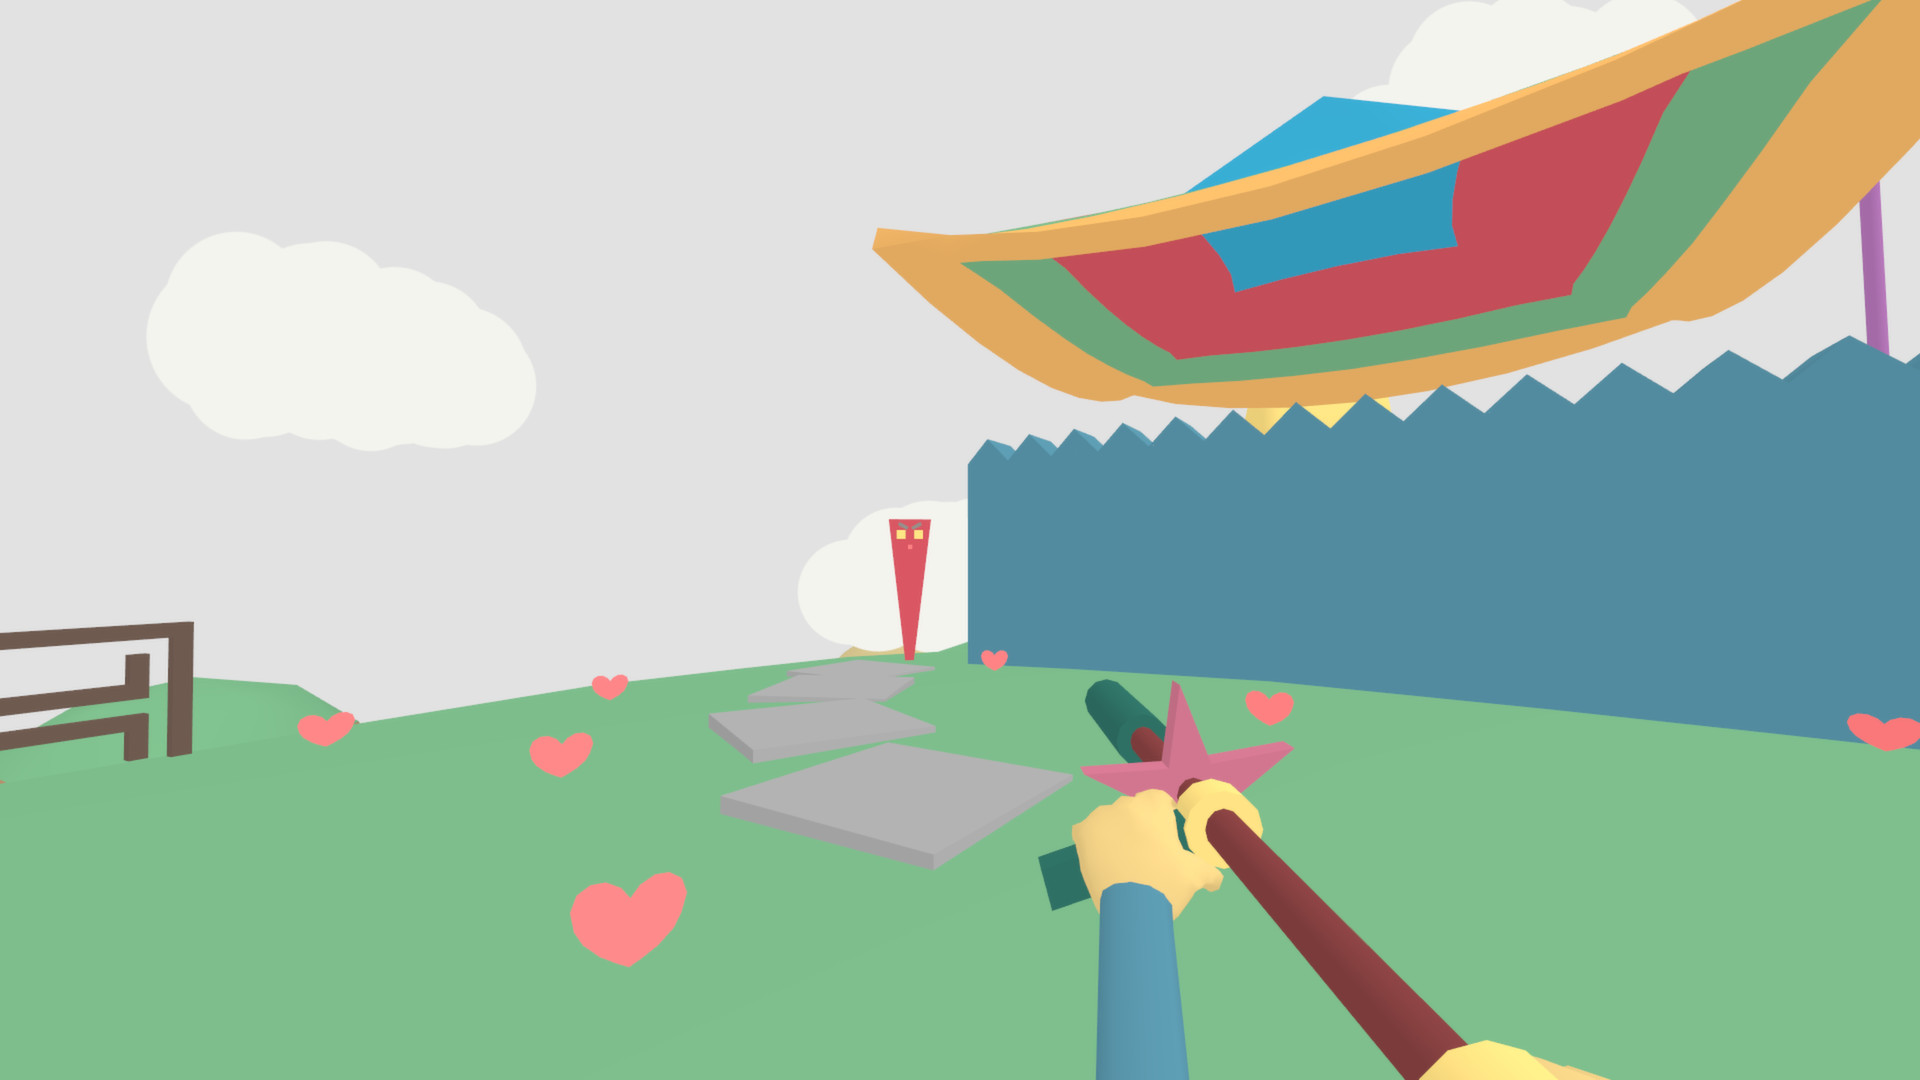
\includegraphics[width=0.88\linewidth]{imgs/lovelyplanet.jpg}
\fonte{imagem de \textit{Lovely Planet} utilizada no TCC1 \cite{LOVELY}}
\end{figure}

% Relatório do TCC2: edição mantida diretamente neste arquivo LaTeX.
\chapter{Materiais e métodos}\label{cap:tcc2-4}

Este capítulo descreve os recursos e procedimentos empregados no desenvolvimento. São apresentadas as ferramentas, a arquitetura de comunicação, as tecnologias de rede, a infraestrutura de observabilidade, a organização do projeto e os métodos de verificação e coleta. Os procedimentos de avaliação são apresentados neste capítulo, enquanto seus registros e resultados são reunidos na seção~\ref{sec:5.3}.

\section{Ferramentas e tecnologias}\label{sec:4.1}

A Godot 4.5 foi utilizada nos projetos Client e Server, com comportamentos programados em GDScript. O Blender integra o fluxo de autoria dos recursos visuais, e o projeto utiliza Git para controle de versão. Scripts PowerShell dão suporte à preparação dos diretórios compartilhados e à sincronização do mapa. Para a dashboard foram utilizados Python e FastAPI, com recepção UDP, comunicação WebSocket e consulta de dados do processo por psutil. A Tabela~\ref{tab:tcc2-1} resume o papel desses materiais.

\begingroup
\small
\setlength{\tabcolsep}{4pt}
\renewcommand{\arraystretch}{1.18}
\begin{longtable}{>{\raggedright\arraybackslash}p{\dimexpr0.32\textwidth-2\tabcolsep\relax}>{\raggedright\arraybackslash}p{\dimexpr0.68\textwidth-2\tabcolsep\relax}}
\caption{Ferramentas e responsabilidades}\label{tab:tcc2-1}\\
\toprule
Material & Utilização no trabalho \\
\midrule
\endfirsthead
\multicolumn{2}{l}{\small Ferramentas e responsabilidades (continuação)}\\
\toprule
Material & Utilização no trabalho \\
\midrule
\endhead
\midrule
\multicolumn{2}{r}{\small Continua na próxima página.}\\
\endfoot
\bottomrule
\endlastfoot
Godot e GDScript & Cenas, física, regras, interface, áudio e comunicação do jogo. \\
Blender & Autoria e manutenção dos modelos e recursos visuais. \\
Git & Organização e versionamento do projeto. \\
PowerShell & Preparação dos links compartilhados e geração de cenas do mapa de servidor. \\
Python e FastAPI & Recepção e disponibilização das amostras na dashboard. \\
psutil & Consulta de CPU e memória do processo identificado pelo PID. \\
\end{longtable}
\endgroup

Fonte: elaboração própria.

\section{Arquitetura e tecnologias de rede}\label{sec:4.2}

\subsection{Arquitetura de comunicação}\label{sec:4.2.1}

A arquitetura define como os participantes trocam informações e onde são decididos os resultados. Fiedler apresenta tanto a troca de comandos entre pares quanto a organização cliente-servidor. Nesta última, o servidor mantém uma referência comum para os clientes; no modelo de simulação determinística entre pares, a reprodução consistente dos comandos depende de condições iniciais e regras equivalentes. Esses modelos exigem soluções diferentes para sincronização. \cite{FIEDLER-REDE}

No projeto, adotou-se um processo servidor separado dos programas executados pelos jogadores. A entrada e a movimentação permanecem no Client, enquanto dano, recursos e pontuação são decididos pelo Server. Essa divisão combina resposta local ao controle com uma referência comum para os resultados das partidas. A organização dos componentes e o alcance dessa autoridade são detalhados na seção~\ref{sec:5.2}.

\subsection{Tecnologias de comunicação utilizadas}\label{sec:4.2.2}

O UDP é um protocolo de transporte baseado em datagramas. Sua especificação não garante entrega nem proteção contra duplicação de mensagens; requisitos adicionais devem ser tratados por outras camadas. No trabalho, ele aparece em dois contextos: como base da comunicação multijogador por ENet e como transporte direto das amostras enviadas à dashboard. A escolha do transporte, por si só, não determina se uma mensagem da aplicação será reenviada. \cite{UDP} \cite{GODOT-REDE}

A Godot disponibiliza comunicação de alto nível por chamadas remotas de procedimento, ou RPCs. Uma função pode ser executada em outro participante, com restrições sobre quem pode chamá-la e sobre a forma de transferência. Essa API permite usar a estrutura de nós do jogo para organizar a comunicação; o projeto a utiliza nos componentes que representam o servidor e cada lobby. \cite{GODOT-REDE}

Os modos de transferência usados são confiável, não confiável e não confiável ordenado. No primeiro, há confirmação e tentativas de reenvio; no segundo, uma mensagem pode se perder ou chegar fora de ordem; no terceiro, mensagens atrasadas podem ser descartadas quando uma atualização posterior já foi recebida. Essa diferença fundamenta o uso de eventos confiáveis para mudanças discretas e de atualizações substituíveis para movimento. \cite{GODOT-PEER}

Outra técnica utilizada foi a interpolação de snapshots. Um snapshot é um registro do estado em determinado instante. Ao manter um pequeno histórico dos registros recebidos, o Client pode apresentar uma posição intermediária entre dois deles, em vez de saltar diretamente para cada atualização. O buffer acrescenta um atraso de apresentação, em troca de uma transição visual mais contínua. \cite{FIEDLER-INTERPOLACAO}

\section{Observabilidade}\label{sec:4.3}

A observabilidade utiliza informações produzidas por um sistema para ajudar a compreender seu comportamento. A documentação do OpenTelemetry apresenta métricas como medições que descrevem aspectos de sua operação. No contexto deste jogo, elas permitem acompanhar condições como quantidade de participantes, tráfego de rede e tempo de execução de uma parte do servidor. O projeto possui instrumentação própria; não utiliza uma integração com o OpenTelemetry. \cite{OBSERVABILIDADE}

A infraestrutura combina apresentação em tempo real e gravação em CSV. A primeira permite acompanhar uma partida enquanto ocorre; a segunda preserva amostras para análise posterior. Para comparar condições de execução, o protocolo da seção~\ref{sec:4.8} prevê registrar o cenário, o intervalo de coleta e a origem dos indicadores.

\section{Processo de desenvolvimento}\label{sec:4.4}

O planejamento original do TCC1 adotou o Double Diamond como referência de processo. O modelo apresentado pelo Design Council organiza atividades de descoberta, definição, desenvolvimento e entrega. Neste trabalho, ele contextualiza o planejamento inicial, sem caracterizar um protocolo de avaliação das iterações realizadas. \cite{DOUBLE-DIAMOND}

O desenvolvimento integrou progressivamente os sistemas de jogador, combate, modos de partida, interface e observabilidade. O relatório apresenta essa organização por responsabilidades, relacionando as soluções adotadas aos problemas de interação e sincronização. A evolução do escopo é discutida na seção seguinte, e o funcionamento dos sistemas é detalhado no capítulo~\ref{cap:tcc2-5}.

\section{Evolução da proposta do TCC1}\label{sec:4.5}

A proposta original previa um participante hospedeiro e utilizava a denominação peer-to-peer para sua arquitetura. A implementação passou a separar o programa executado pelos jogadores do processo que mantém as partidas. Essa mudança permitiu executar o Server sem a apresentação do jogo e manter em um ponto comum as regras de dano, recursos, modos e resultados. RPCs e snapshots próprios substituíram a dependência do mecanismo de replicação automática descrito no protótipo inicial, tornando explícitas as responsabilidades de cada lado da comunicação.

A configuração livre por um jogador hospedeiro também foi substituída por presets compartilhados. Com isso, Client e Server trabalham com combinações previamente conhecidas de mapa, modo, tempo, pontuação e quantidade de participantes, e o gerenciador pode associar solicitações compatíveis ao mesmo lobby. Essa delimitação reduz as variações que precisam ser tratadas e verificadas na versão entregue.

O recorte de conteúdo foi ajustado para concentrar o desenvolvimento e a verificação em um conjunto menor de combinações. Foram disponibilizados TDM e KOTH em Highrise, enquanto Capture the Flag e o mapa Prototype ficaram fora da seleção principal. Highrise passou a reunir os elementos necessários aos dois modos entregues, como pontos de nascimento, recursos, jump pads e zona de controle. Dessa forma, o mesmo mapa pode ser utilizado no fluxo principal e nas duas modalidades disponíveis.

O catálogo final de combate também foi revisto. Pistola, SMG e shotgun assumem papéis diferenciados por cadência, dispersão e quantidade de traços, enquanto as granadas acrescentam dano em área. A melhoria de velocidade de movimentação prevista inicialmente deu lugar ao aumento temporário de cadência, integrado ao mesmo ciclo de armas, munição e feedback da interface. Essas alterações descrevem o produto efetivamente consolidado e são sintetizadas na seção~\ref{sec:5.3.3}.

\section{Organização do projeto}\label{sec:4.6}

O projeto foi organizado em dois projetos Godot independentes, Client e Server, e um diretório de código comum, \texttt{shared}. Essa estrutura permite executar o servidor separadamente da apresentação do jogo e reutilizar contratos de comunicação e definições nos dois lados. A Figura~\ref{fig:tcc2-2} apresenta os principais agrupamentos de responsabilidades, cujo funcionamento é discutido no relatório técnico.

O compartilhamento local é preparado por um script que cria links de diretório para uma mesma origem, evitando cópias independentes das definições comuns. Os arquivos de autoria dos assets são mantidos em pastas \texttt{import/}. A preparação desses recursos compõe o procedimento de geração dos executáveis descrito na seção~\ref{sec:5.2.11}.

Este relatório descreve a versão do projeto preparada para entrega. O código-fonte e a documentação técnica complementar estão disponíveis em \url{https://github.com/limaalan/TCC}. O Apêndice~\ref{ap:fontes-tecnicas} reúne os caminhos de consulta desse material.

\section{Método de verificação funcional}\label{sec:4.7}

A verificação funcional prevê executar o Server e conectar dois Clients, percorrendo o fluxo completo de partida. O roteiro inclui entrada no lobby, escolha de modo, nascimento dos personagens, combate, coleta de recursos, atualização da interface, encerramento e retorno ao menu. Para KOTH, é necessário observar separadamente a zona vazia, controlada e contestada, pois cada estado produz uma consequência diferente sobre a pontuação.

O registro do teste deve identificar a data, a plataforma, os executáveis utilizados e o resultado observado em cada cenário. A Tabela~\ref{tab:tcc2-5} organiza os comportamentos implementados e as situações que precisam ser exercitadas na versão preparada para entrega. Sua aprovação depende dos registros de execução, ainda assinalados como pendentes.

\begin{quote}
\small
\textbf{Evidência pendente:} registro do teste integrado da versão escolhida para a entrega, com data, identificação da build, participantes ou instâncias utilizadas e resultado de cada cenário. O procedimento acima está definido; sua aprovação não foi presumida.
\end{quote}

\section{Método de coleta e análise de métricas}\label{sec:4.8}

A infraestrutura de métricas permite coletar amostras periódicas, com intervalo padrão de um segundo, e gravá-las em CSV ou transmiti-las à dashboard. O coletor utiliza contadores do host ENet, estatísticas dos peers e informações de lobbies e jogadores. Os Clients também informam seus FPS, que são reunidos pelo Server. Essa infraestrutura fornece as variáveis para o experimento, mas a quantidade de amostras e a duração efetiva de cada rodada precisam ser registradas durante sua execução.

Para a avaliação desta versão, propõe-se comparar o servidor sem partidas ativas com uma partida de dois jogadores em TDM e uma de dois jogadores em KOTH. Cada rodada deve usar a mesma build, intervalo de coleta e ambiente, registrando o período de espera e o de jogo ativo. Experimentos com mais lobbies podem ampliar essa comparação até o limite configurado, desde que sejam identificados separadamente. Esse protocolo orienta a avaliação quantitativa e mantém as condições comparáveis entre os dois modos.

A análise deverá relacionar tráfego, RTT, perda estimada de pacotes e tempo medido do processamento dos lobbies ao número de participantes e ao estado da partida. Para evitar comparar medidas diferentes, devem ser preservados os nomes, as unidades e os timestamps do contrato. A medição de CPU e memória requer um registro adicional: esses valores são consultados pela dashboard no sistema operacional e não integram automaticamente os CSVs produzidos pelo logger do Godot.

\begin{quote}
\small
\textbf{Evidência pendente:} ambiente de execução, duração e repetições das rodadas, arquivos de dados brutos e resultados calculados. Não foram atribuídos valores a latência, CPU, memória ou capacidade do servidor sem essas medições.
\end{quote}

% Texto adaptado de docs/tcc2/relatorio_tcc2.md para a prévia do TCC2.
\chapter{Desenvolvimento e resultados}\label{cap:tcc2-5}

Este capítulo apresenta o produto desenvolvido e os resultados disponíveis. A primeira parte descreve a experiência do ponto de vista do jogador, funcionando como um guia conciso do jogo entregue. A segunda constitui o relatório técnico, no qual são discutidas a arquitetura, a sincronização e a implementação das principais funcionalidades. A parte final reúne a verificação funcional, os resultados das métricas, a comparação com a proposta e as limitações identificadas.

\section{Visão geral do jogo final}\label{sec:5.1}

Esta seção apresenta o jogo conforme percebido pelo participante, desde a entrada em uma partida até a exibição do resultado. Os detalhes internos que sustentam esse funcionamento são discutidos posteriormente, no relatório técnico.

\subsection{Conceito e ciclo principal de jogabilidade}\label{sec:5.1.1}

O jogo desenvolvido organiza confrontos entre duas equipes em uma arena tridimensional. O participante informa seu nome, seleciona um preset e aguarda a formação da partida. Após o carregamento do mapa e a escolha de arma, passa a controlar seu personagem, podendo buscar recursos, enfrentar o adversário e disputar o objetivo do modo. A partida termina conforme suas regras, e uma tela apresenta os resultados por equipe e por jogador. \fonteprojeto{PRESETS} \fonteprojeto{SERVER} \fonteprojeto{SERVER-LOBBY} \fonteprojeto{MENU} \fonteprojeto{RESULTADO}

O ciclo de interação combina deslocamento, gerenciamento de munição e confronto. Ao perder todos os pontos de vida, o personagem é removido e, caso a partida continue, o jogador recebe uma nova oportunidade de escolher sua arma e retornar ao mapa. Dessa forma, a participação se organiza em torno da disputa em andamento. O inventário é preparado novamente no nascimento, sem representar uma progressão persistente entre partidas. \fonteprojeto{SERVER-LOBBY} \fonteprojeto{INVENTARIO}

\subsection{Controles e movimentação}\label{sec:5.1.2}

A movimentação foi implementada no Client por meio de um corpo tridimensional controlado por script. A direção é calculada a partir da entrada e da orientação do personagem. A câmera permite olhar horizontal e verticalmente, com limitação da rotação vertical. O jogador pode correr e realizar até dois saltos antes de retornar ao chão. A implementação também considera a entrada por controle, incluindo deslocamento e mira pelos analógicos. \fonteprojeto{JOGADOR-LOCAL} \fonteprojeto{PROJETO-CLIENT}

O salto duplo é controlado por uma contagem de saltos utilizados. Quando o personagem aterrissa, essa contagem é reiniciada; ao tocar uma plataforma de impulso, a velocidade vertical é alterada e os saltos também são restabelecidos. Os jump pads são configurados pelo Server e apresentados no Client, onde a detecção de contato aplica o impulso ao personagem local. O Server recebe depois a posição resultante pelo fluxo normal de movimento; não há uma validação separada de cada impulso na implementação consultada. \fonteprojeto{JOGADOR-LOCAL} \fonteprojeto{JUMP-PAD} \fonteprojeto{SERVER-LOBBY}

\begingroup
\small
\setlength{\tabcolsep}{4pt}
\renewcommand{\arraystretch}{1.18}
\begin{longtable}{>{\raggedright\arraybackslash}p{\dimexpr0.23\textwidth-2\tabcolsep\relax}>{\raggedright\arraybackslash}p{\dimexpr0.35\textwidth-2\tabcolsep\relax}>{\raggedright\arraybackslash}p{\dimexpr0.42\textwidth-2\tabcolsep\relax}}
\caption{Principais controles presentes na configuração do Client}\label{tab:tcc2-2}\\
\toprule
Ação & Teclado e mouse & Controle, em nomenclatura equivalente à disposição Xbox \\
\midrule
\endfirsthead
\multicolumn{3}{l}{\small Principais controles presentes na configuração do Client (continuação)}\\
\toprule
Ação & Teclado e mouse & Controle, em nomenclatura equivalente à disposição Xbox \\
\midrule
\endhead
\midrule
\multicolumn{3}{r}{\small Continua na próxima página.}\\
\endfoot
\bottomrule
\endlastfoot
Movimentar & W, A, S e D & Analógico esquerdo \\
Mirar & Movimento do mouse & Analógico direito \\
Correr & Shift & Pressionar o analógico esquerdo \\
Saltar & Espaço & A \\
Disparar & Botão esquerdo do mouse & Gatilho direito ou botão superior direito \\
Lançar granada & Q & Botão superior esquerdo ou B \\
Selecionar arma & 1, 2 e 3 & Direcional esquerdo/direito para alternar \\
Abrir ou fechar pausa & Esc & Start/Menu \\
\end{longtable}
\endgroup

Fonte: Input Map e tratamento de entrada do Client. O mapeamento documenta a configuração existente; a verificação em dispositivos físicos integra o teste da release. \fonteprojeto{PROJETO-CLIENT} \fonteprojeto{JOGADOR-LOCAL} \fonteprojeto{GUIA-RELEASE}

\subsection{Fluxo de telas}\label{sec:5.1.3}

O gerenciador de cenas abre o menu principal quando o Client inicia. A formação da partida conduz ao carregamento do mapa e à seleção de arma; durante o jogo, a pausa disponibiliza uma tela local e libera o cursor. Esse estado interrompe o controle daquele jogador, mas não suspende o processo servidor. Ao final da partida, os dados recebidos são entregues à tela de resultado, que permite voltar ao menu. A Figura~\ref{fig:tcc2-1} resume esse encadeamento. \fonteprojeto{CENAS-CLIENT} \fonteprojeto{JOGADOR-LOCAL} \fonteprojeto{CLIENT-LOBBY} \fonteprojeto{RESULTADO}

\begin{figure}[htbp]
\centering
\caption{Fluxo principal de telas e participação}
\label{fig:tcc2-1}
% Fluxo de telas do jogo.
\resizebox{0.96\linewidth}{!}{%
\begin{tikzpicture}[
  bloco/.style={draw,rounded corners,align=center,text width=2.8cm,minimum height=.75cm,font=\small},
  seta/.style={-{Latex[length=2mm]},thick}
]
\node[bloco] (menu) at (0,0) {Menu principal};
\node[bloco] (espera) at (0,-1.2) {Espera por partida};
\node[bloco] (mapa) at (0,-2.4) {Carregamento do mapa};
\node[bloco] (arma) at (0,-3.6) {Seleção de arma};
\node[bloco] (partida) at (0,-4.8) {Partida e HUD};
\node[bloco] (pausa) at (-4,-4.8) {Pausa local};
\node[bloco] (morte) at (4,-4.8) {Morte e espera};
\node[bloco] (resultado) at (0,-6.2) {Resultado};
\draw[seta] (menu) -- (espera);
\draw[seta] (espera) -- (mapa);
\draw[seta] (mapa) -- (arma);
\draw[seta] (arma) -- (partida);
\draw[seta] (partida) to[bend right=15] (pausa);
\draw[seta] (pausa) to[bend right=15] (partida);
\draw[seta] (partida) -- (morte);
\draw[seta] (morte) |- (arma);
\draw[seta] (partida) -- (resultado);
\draw[seta] (resultado.south) -- ++(0,-.6) -- (-6,-6.8) -- (-6,0) -- (menu.west);
\end{tikzpicture}%
}

\fonte{elaboração a partir dos gerenciadores de cena e lobby. O retorno após a morte depende de a partida continuar ativa. \fonteprojeto{CENAS-CLIENT} \fonteprojeto{CLIENT-LOBBY} \fonteprojeto{SERVER-LOBBY}}
\end{figure}

\subsection{Modos de jogo e objetivos}\label{sec:5.1.4}

O jogador pode participar de Team Deathmatch ou King of the Hill. No primeiro modo, as equipes disputam pontos por meio das eliminações, e quedas que provoquem a morte também favorecem a equipe adversária. No segundo, o objetivo é ocupar a zona demarcada no mapa: uma equipe pontua enquanto controla sozinha a região, e a progressão é interrompida quando adversários entram na área. \fonteprojeto{TDM} \fonteprojeto{KOTH} \fonteprojeto{COLINA} \fonteprojeto{ZONA-MORTE}

Nos presets disponíveis, as partidas utilizam meta de 20 pontos e duração máxima de 300 segundos. Ao atingir a meta ou terminar o tempo, o jogo apresenta a equipe vencedora e os dados individuais dos participantes. \fonteprojeto{PRESETS} \fonteprojeto{RESULTADO}

\subsection{Armas, granadas e recursos da arena}\label{sec:5.1.5}

O arsenal é formado por pistola, SMG e shotgun. A pistola realiza disparos individuais, a SMG permite manter o gatilho pressionado e a shotgun dispara vários traços simultaneamente. O jogador escolhe uma arma antes de entrar ou retornar à arena e precisa administrar sua munição durante a partida. Também pode lançar granadas, que explodem após um intervalo e causam dano de acordo com a distância. \fonteprojeto{ARMAS} \fonteprojeto{PISTOLA} \fonteprojeto{SMG} \fonteprojeto{SHOTGUN} \fonteprojeto{GRANADA-SERVER}

O mapa distribui pickups de vida, munição e granadas, além de dois power-ups temporários. Um deles aumenta o dano dos disparos e o outro reduz o intervalo entre tiros. Depois de coletados, os recursos permanecem indisponíveis por um período antes de reaparecerem. \fonteprojeto{PICKUPS} \fonteprojeto{BUFF-DANO} \fonteprojeto{BUFF-CADENCIA}

\subsection{Interface e feedback ao jogador}\label{sec:5.1.6}

A HUD informa vida, equipe, arma equipada, munição, granadas e efeitos temporários. Durante a partida, também apresenta o tempo, o placar e, em KOTH, o estado da zona de controle. Cores, anéis e ícones auxiliam na identificação das equipes. \fonteprojeto{HUD-CENA} \fonteprojeto{JOGADOR-LOCAL} \fonteprojeto{CLIENT-LOBBY}

Sons, recuo, efeitos de disparo e impacto e alterações visuais dos personagens complementam essas informações. Esses sinais permitem perceber a ocorrência de ações como disparos, coletas, explosões e recebimento de dano sem depender exclusivamente de mensagens textuais. \fonteprojeto{AUDIO} \fonteprojeto{DISPARO-LOCAL} \fonteprojeto{PERSONAGEM} \fonteprojeto{ROSTO}

\section{Relatório técnico}\label{sec:5.2}

Esta seção concentra a descrição do desenvolvimento. A organização acompanha as responsabilidades e relações entre os sistemas, utilizando as funcionalidades como exemplos da solução técnica em vez de enumerar arquivos e classes.

\subsection{Separação entre Client, Server e shared}\label{sec:5.2.1}

O sistema foi dividido para que apresentação e regras de partida pudessem ser executadas em processos diferentes. O Client recebe a entrada, movimenta o personagem local e apresenta modelos, sons e interface. O Server organiza os participantes e mantém os estados utilizados no combate, na coleta de itens e na pontuação. O diretório \texttt{shared} contém definições comuns, evitando que identificadores e regras como os limites de munição sejam mantidos de forma independente nos dois projetos. \fonteprojeto{DOC-ARQUITETURA} \fonteprojeto{DOC-SHARED} \fonteprojeto{INVENTARIO}

\begin{figure}[htbp]
\centering
\caption{Responsabilidades dos componentes. \texttt{shared} é um diretório de código e recursos, e não um serviço da rede}
\label{fig:tcc2-2}
% shared representa arquivos usados pelos dois projetos, não um serviço.
\resizebox{0.96\linewidth}{!}{%
\begin{tikzpicture}[
  bloco/.style={draw,rounded corners,align=center,text width=4.5cm,minimum height=1.3cm,font=\small},
  seta/.style={-{Latex[length=2mm]},thick}
]
\node[bloco] (client) at (-4,0) {Client\\Entrada, movimento local\\e apresentação};
\node[bloco] (server) at (4,0) {Server\\Lobbies, combate,\\recursos e modos};
\node[bloco] (shared) at (0,3.1) {shared\\Contratos, presets e definições};
\draw[seta] (client.north east) -- node[above,align=center,font=\footnotesize] {Estado local\\e solicitações} (server.north west);
\draw[seta] (server.south west) -- node[below,font=\footnotesize] {Snapshots e eventos} (client.south east);
\draw[seta,dashed] (shared) -- node[left,font=\footnotesize] {Usado pelo código} (client);
\draw[seta,dashed] (shared) -- node[right,font=\footnotesize] {Usado pelo código} (server);
\end{tikzpicture}%
}

\fonte{organização dos projetos e fluxo dos lobbies. \fonteprojeto{DOC-SHARED} \fonteprojeto{CLIENT-LOBBY} \fonteprojeto{SERVER-LOBBY}}
\end{figure}

\subsection{Comunicação e autoridade do servidor}\label{sec:5.2.2}

O disparo exemplifica essa divisão. O Client apresenta o efeito local e envia a solicitação. O Server verifica se o jogador possui uma instância ativa, identifica a arma registrada e tenta consumir a munição correspondente. Se houver saldo, calcula os acertos e aplica o dano. As alterações de vida e os efeitos de impacto são então comunicados aos participantes. A apresentação imediata do disparo não concede ao Client a responsabilidade de decidir quem foi atingido. \fonteprojeto{DISPARO-LOCAL} \fonteprojeto{SERVER-LOBBY} \fonteprojeto{CLIENT-LOBBY}

A autoridade implementada possui limites. O Server aceita a transformação enviada pelo jogador após verificar a estrutura da mensagem, e o caminho de recepção do disparo não contém uma verificação explícita de intervalo mínimo entre solicitações. O cooldown e seu multiplicador de cadência são aplicados no Client. Assim, dano e munição são decididos no Server, mas a versão atual não equivale a uma validação completa de movimento e frequência de tiro contra um Client modificado. \fonteprojeto{SERVER-LOBBY} \fonteprojeto{DISPARO-LOCAL} \fonteprojeto{PERSONAGEM}

\subsection{Sessões, lobbies e presets de partida}\label{sec:5.2.3}

Uma conexão ao servidor e a participação em uma partida são estados diferentes. O Server recebe conexões e procura um lobby disponível para o preset solicitado. Quando necessário e permitido pelo limite configurado, cria outro lobby; quando o grupo está completo, inicia a preparação dos Clients. Os presets agrupam modo, mapa, tempo, pontuação e quantidade de participantes, tornando a configuração conhecida pelos dois lados. \fonteprojeto{SERVER} \fonteprojeto{PRESETS}

Na configuração consultada, o peer aceita até 64 conexões, o gerenciador possui quatro posições de lobby e cada preset utiliza dois jogadores. Portanto, o limite de conexões não significa 64 jogadores na mesma partida. Cada lobby mantém seus próprios participantes e estado, e suas cenas são posicionadas com uma separação espacial no processo servidor. A comprovação de execução simultânea dos quatro lobbies exige um cenário de avaliação próprio. \fonteprojeto{SERVER} \fonteprojeto{PRESETS} \fonteprojeto{SERVER-LOBBY}

\subsection{Sincronização de rede}\label{sec:5.2.4}

\textbf{Envio contínuo de movimento.} A cada ciclo de física, o Client envia posição, rotação horizontal, inclinação da mira e animação. O Server copia esses dados para a representação do jogador e os utiliza na composição do estado da partida. Esse envio emprega o modo não confiável ordenado, adequado ao tratamento de informações que serão substituídas por novas atualizações. O fluxo transmite o resultado local do movimento, em vez de uma sequência de comandos para o Server simular novamente. \fonteprojeto{CLIENT-LOBBY} \fonteprojeto{SERVER-LOBBY}

\subsubsection{Interpolação dos estados remotos}\label{sec:5.2.4.1}

O Server distribui snapshots do estado do mundo a cada três ciclos de física, enquanto o Client produz novos quadros continuamente. Como o tempo de trânsito pela rede pode variar, os snapshots podem chegar em intervalos irregulares. Se cada quadro utilizasse apenas o estado mais recente, uma renderização poderia ocorrer antes da chegada da atualização seguinte, mantendo temporariamente a última posição conhecida ou exigindo uma estimativa do movimento. \fonteprojeto{SERVER-LOBBY} \fonteprojeto{CLIENT-LOBBY}

Para reduzir essas descontinuidades, o Client mantém um buffer e calcula um instante de apresentação 100 milissegundos no passado. O desvio estimado entre os relógios do Client e do Server também participa desse cálculo. A cada quadro, o sistema procura dois estados conhecidos ao redor do instante de apresentação e interpola entre eles as posições e rotações dos jogadores remotos. \fonteprojeto{CONEXAO-CLIENT} \fonteprojeto{CLIENT-LOBBY} \fonteprojeto{JOGADOR-REMOTO}

A Figura~\ref{fig:tcc2-3} compara os dois casos com o mesmo conjunto de snapshots disponíveis, posicionados na linha do tempo pelo timestamp do Server, e não pelo instante de chegada ao Client. Sem atraso de apresentação, o instante desejado de 10,000 segundos está além do último estado conhecido, sem um estado posterior para formar o par de interpolação. Com o buffer de 100 milissegundos, o instante de apresentação $R$ passa a ser 9,900 segundos, entre os estados S1 e S2, permitindo calcular uma posição intermediária. Os valores temporais do diagrama são ilustrativos.

\begin{figure}[htbp]
\centering
\caption[Interpolação de snapshots com buffer de apresentação]{Interpolação de snapshots: comparação entre a apresentação sem atraso e com buffer de 100 milissegundos}
\label{fig:tcc2-3}
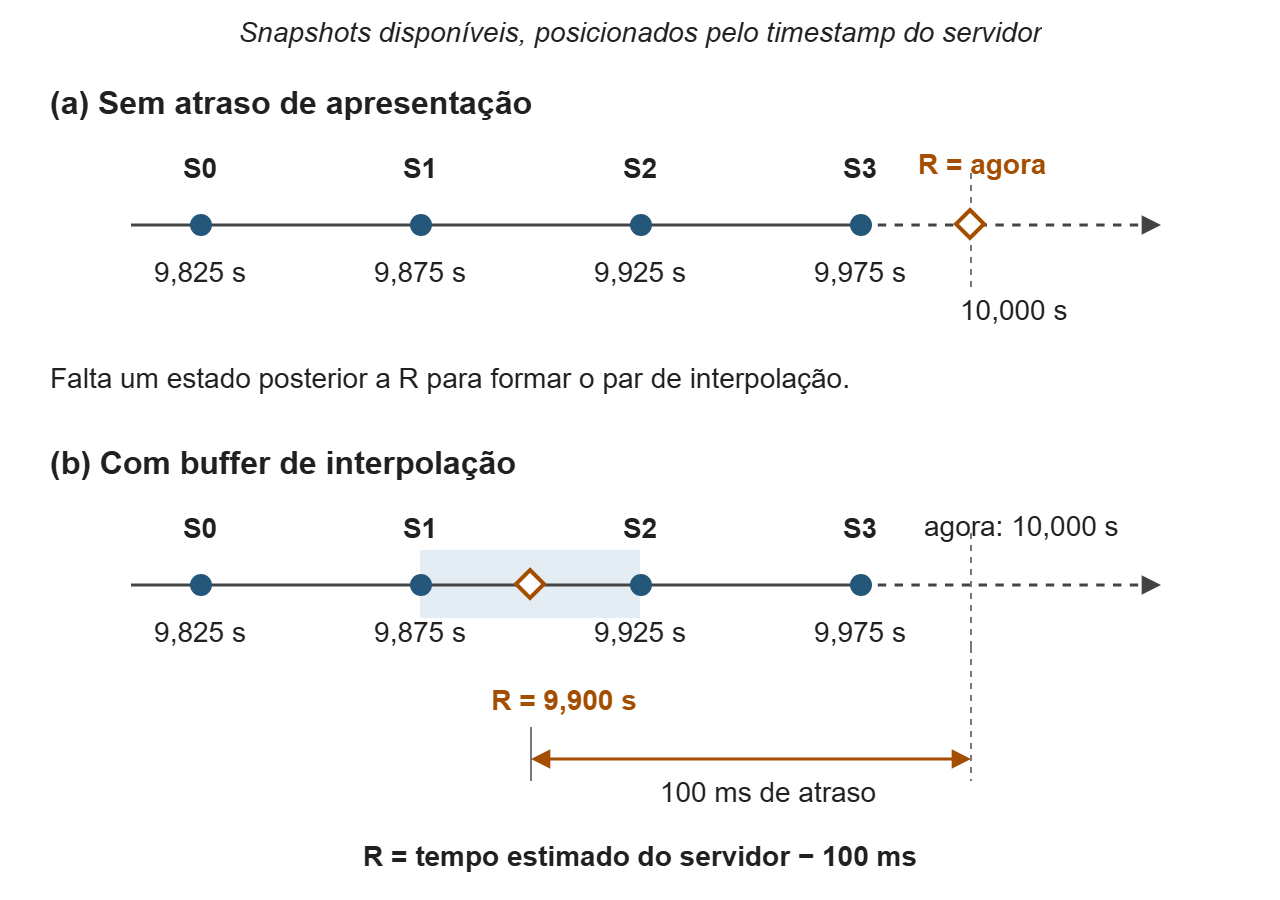
\includegraphics[width=\linewidth,height=0.70\textheight,keepaspectratio]{figuras/tcc2/interpolacao-snapshots.png}
\fonte{elaboração própria a partir da implementação. \fonteprojeto{CLIENT-LOBBY}}
\end{figure}

O atraso de 100 milissegundos é intencional e pertence à apresentação visual; ele não representa uma medição da latência da conexão. Essa estratégia troca uma pequena quantidade fixa de atraso por maior continuidade visual. Na implementação atual, o fator de interpolação não é limitado explicitamente ao intervalo entre zero e um. Caso não exista um estado posterior adequado, o cálculo não garante que o resultado permaneça estritamente entre os dois snapshots utilizados. \fonteprojeto{CLIENT-LOBBY}

\subsubsection{Compensação de latência dos disparos}\label{sec:5.2.4.2}

A interpolação melhora a apresentação dos jogadores remotos, mas não resolve o intervalo entre um disparo no Client e seu processamento pelo Server. Durante esse período, um alvo pode se deslocar. Se o raycast fosse executado somente contra a posição corrente no momento da recepção, um disparo alinhado com aquilo que o atirador viu poderia ser considerado uma falha.

Ao disparar, o Client envia uma referência temporal ajustada pelo desvio estimado entre os relógios. O Server mantém um histórico recente dos estados e, ao receber a solicitação, subtrai os 100 milissegundos do buffer de apresentação para determinar o instante que se aproxima daquele exibido ao atirador. Em seguida, reposiciona as representações auxiliares dos jogadores com os dados históricos, aguarda um ciclo de física e executa o raycast nessa configuração. \fonteprojeto{CONEXAO-CLIENT} \fonteprojeto{CLIENT-LOBBY} \fonteprojeto{SERVER-LOBBY}

A Figura~\ref{fig:tcc2-4} ilustra o processo com todos os instantes expressos na referência temporal do Server. O Client dispara em 10,000 segundos enquanto apresenta aproximadamente o estado A, associado a 9,900 segundos. No exemplo, a solicitação leva 60 milissegundos para chegar ao Server, que já está no estado C em 10,060 segundos. A consulta histórica utiliza o timestamp do disparo menos o buffer visual, isto é, $10{,}000 - 0{,}100 = 9{,}900$ segundos, e não o instante de recepção menos esse buffer. Os 60 milissegundos representam apenas o trânsito de ida em um exemplo ilustrativo, não uma medição nem o tempo de ida e volta da conexão. O estado histórico selecionado aproxima a situação apresentada ao atirador; a implementação não interpola os estados desse histórico.

\begin{figure}[htbp]
\centering
\caption[Compensação de latência na validação de disparos]{Compensação de latência: relação entre o disparo, a recepção e a consulta histórica para validação por raycast}
\label{fig:tcc2-4}
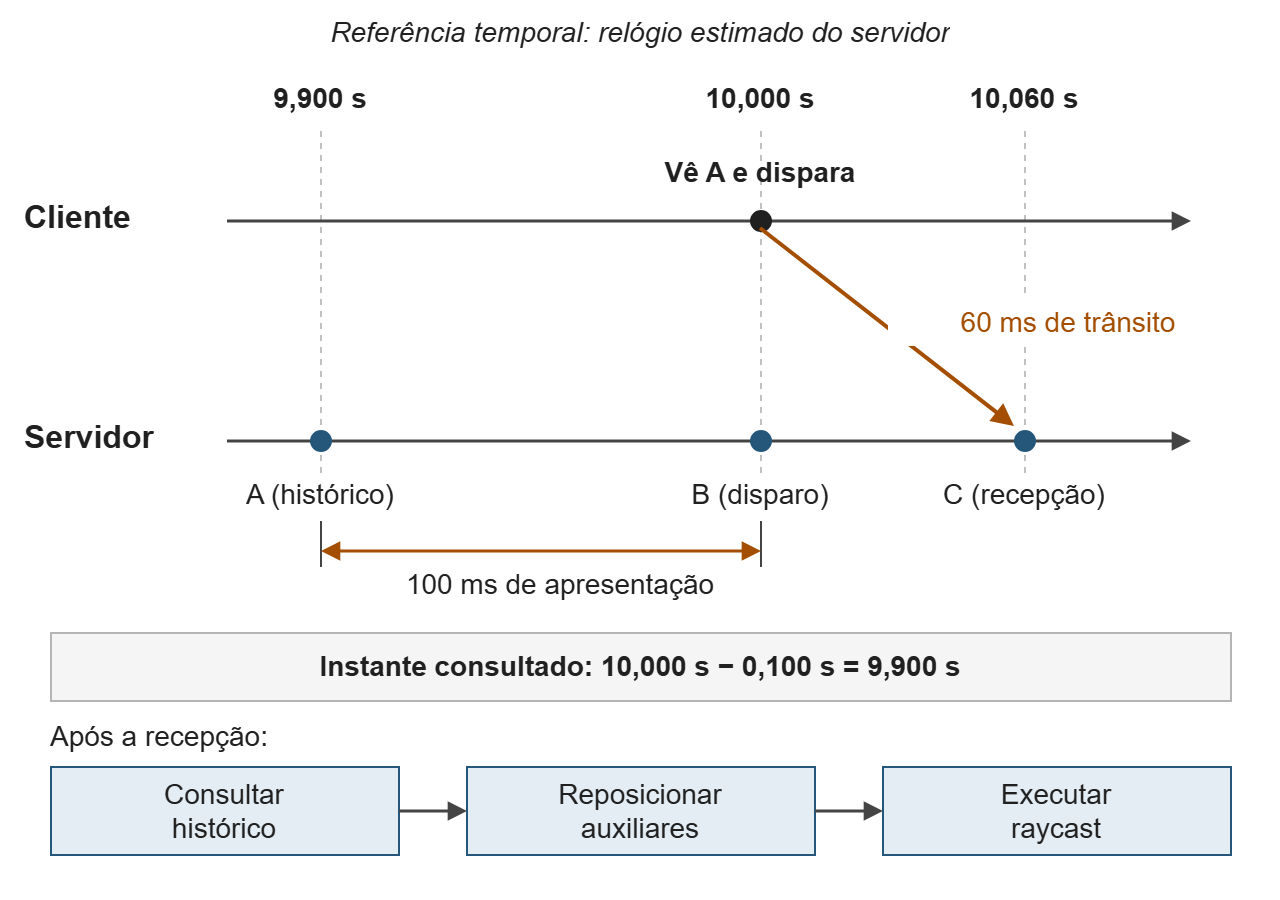
\includegraphics[width=\linewidth,height=0.70\textheight,keepaspectratio]{figuras/tcc2/compensacao-latencia-disparos.png}
\fonte{elaboração própria a partir da implementação. \fonteprojeto{SERVER-LOBBY}}
\end{figure}

Esse procedimento pode ser entendido como uma consulta ao passado para validar o disparo, mas não realiza um rollback completo da partida. O estado corrente do mundo não é integralmente reconstruído nem simulado novamente. Somente as representações auxiliares usadas nos testes de colisão são reposicionadas a partir do histórico recente. O mecanismo busca aproximar a decisão autoritativa da situação vista pelo jogador, sem garantir sincronização exata entre os relógios. \fonteprojeto{SERVER-LOBBY} \fonteprojeto{CONEXAO-CLIENT}

\textbf{Sincronização inicial do mapa.} O Client recebe o identificador do mapa e carrega sua cena local. Após confirmar o carregamento, recebe mensagens confiáveis para criar pickups, objetivos e plataformas especiais. São enviados identificadores e parâmetros de criação, sem retransmitir continuamente toda a geometria visual. Assim, a posição inicial da zona de KOTH e dos jump pads faz parte da preparação da partida. \fonteprojeto{SERVER-LOBBY} \fonteprojeto{CLIENT-LOBBY} \fonteprojeto{PAYLOADS}

\textbf{Atualizações do objetivo.} A criação inicial da zona de controle não elimina a necessidade de comunicar suas mudanças. O KOTH verifica a ocupação durante a execução e transmite o estado da colina a cada 0,25 segundo. A mensagem contém a condição da zona, o time controlador e os jogadores presentes. O placar possui outro fluxo de atualização, permitindo distinguir a existência do objetivo, seu estado atual e a pontuação acumulada. \fonteprojeto{KOTH} \fonteprojeto{COLINA} \fonteprojeto{CLIENT-LOBBY}

\textbf{Eventos confiáveis.} Nascimento, troca de arma, início e término de power-ups e encerramento da partida são comunicados por eventos confiáveis. Nesses casos, a mudança é transmitida quando ocorre, com os dados necessários à atualização da cópia local. O objetivo é preservar a entrega e a ordem enquanto a conexão permanece válida; isso não constitui, por si só, um mecanismo de persistência ou recuperação após desconexão. \fonteprojeto{SERVER-LOBBY} \fonteprojeto{CLIENT-LOBBY} \cite{GODOT-PEER}

\textbf{Predição local e correção de munição.} Ao disparar, o Client reduz sua munição, inicia o cooldown e apresenta recuo, som e efeito de tiro antes da resposta do Server. O valor confirmado pelo servidor substitui a cópia local quando é recebido. Essa antecipação produz uma resposta imediata, mas a implementação não mantém um histórico de comandos confirmados para repetir toda a simulação do personagem. Trata-se de uma correção de estado discreto associada ao disparo. \fonteprojeto{DISPARO-LOCAL} \fonteprojeto{JOGADOR-LOCAL} \fonteprojeto{SERVER-LOBBY}

\textbf{Granadas por snapshots.} As granadas são simuladas fisicamente no Server e identificadas por um código de rede. O Client cria sua representação quando o identificador aparece nos snapshots e interpola as transformações recebidas. A explosão visual ocorre quando a granada desaparece entre dois estados consecutivos. Embora o Server também envie uma notificação confiável de explosão, o handler atual dessa notificação está vazio no Client; a apresentação efetiva depende da transição dos snapshots. \fonteprojeto{GRANADA-SERVER} \fonteprojeto{SERVER-LOBBY} \fonteprojeto{CLIENT-LOBBY}

\textbf{Reenvio do estado atual.} Além das atualizações individuais, o Server pode enviar o inventário completo de munição e os power-ups ativos. No caso de um buff já em andamento, a mensagem de reenvio utiliza duração zero. O Client aplica os multiplicadores e a apresentação do efeito, mas o personagem local somente inicia um temporizador de HUD quando recebe uma duração positiva. Esse fluxo repõe informações atuais sem repetir as coletas anteriores e sem reconstruir o tempo restante do indicador. \fonteprojeto{SERVER-LOBBY} \fonteprojeto{PERSONAGEM} \fonteprojeto{JOGADOR-LOCAL}

\textbf{Eventos visuais e dados substituíveis.} Efeitos remotos de tiro, impacto e coleta utilizam mensagens não confiáveis. Vida, quantidade de granadas e tempo de partida possuem atualizações não confiáveis ordenadas. A perda de uma mensagem de apresentação não modifica o estado calculado no Server, mas pode deixar um indicador desatualizado até uma comunicação posterior. No caso da vida, por exemplo, não se deve presumir uma correção periódica independente se nenhuma nova atualização ocorrer. \fonteprojeto{SERVER-LOBBY} \fonteprojeto{CLIENT-LOBBY}

\textbf{Variações visuais locais.} O time do jogador é enviado na mensagem de criação, mas a variante de cor da skin não faz parte desse contrato. Cada Client escolhe uma cor da paleta correspondente ao criar sua representação remota. Por isso, o mesmo personagem pode ter tonalidades diferentes em computadores distintos. O anel utiliza um material fixo para cada equipe, mantendo essa identificação vinculada ao time recebido. \fonteprojeto{PAYLOADS} \fonteprojeto{JOGADOR-REMOTO}

\textbf{Comparação com simulação determinística e catch-up.} O material Network Weapon with netfox apresenta uma alternativa em que projéteis avançam por passos determinísticos, recuperam passos perdidos por catch-up e reconciliam a posição inicial com a autoridade usando um limiar de distância. Essas estratégias servem como referência conceitual, mas não descrevem os tiros deste projeto: suas armas usam raycasts históricos, e as granadas recebem transformações periódicas. Não se deve confundir a compensação histórica de um acerto com a execução acelerada de passos de um projétil. \cite{NETFOX} \fonteprojeto{SERVER-LOBBY}

\subsection{Jogador, times e ciclo de vida}\label{sec:5.2.5}

Cada participante possui uma representação local em seu Client e representações remotas nos demais. O Server mantém os dados utilizados na partida, incluindo time, arma, vida e estatísticas. A criação transmite essas informações para que cada Client instancie o tipo de personagem adequado. O jogador remoto combina animação corporal e orientação da mira para apresentar o estado recebido pela rede. \fonteprojeto{SERVER-LOBBY} \fonteprojeto{CLIENT-LOBBY} \fonteprojeto{JOGADOR-REMOTO}

A identificação das equipes utiliza materiais do personagem, um anel e um ícone na HUD do jogador local. O ícone permite consultar o próprio time sem depender de enxergar o corpo do personagem em primeira pessoa. As variações de skin permanecem locais, conforme descrito na seção anterior, enquanto a equipe utilizada pelas regras é definida no Server. \fonteprojeto{JOGADOR-REMOTO} \fonteprojeto{JOGADOR-LOCAL}

O jogador possui vida máxima de 100 pontos. Quando o valor chega a zero, o Server remove suas representações, retira sua presença dos objetivos e limpa os power-ups. Se a partida continuar, aguarda cinco segundos antes de solicitar uma nova escolha de arma. O retorno ocorre com a preparação do estado de nascimento e da munição correspondente à escolha, sem um contador de vidas limitado nos presets atuais. \fonteprojeto{JOGADOR-SERVER} \fonteprojeto{SERVER-LOBBY} \fonteprojeto{INVENTARIO} \fonteprojeto{PRESETS}

\subsection{Modos de jogo e fluxo da partida}\label{sec:5.2.6}

\textbf{Team Deathmatch.}

No Team Deathmatch, o objetivo é obter a maior pontuação no confronto entre equipes. Na implementação, a pontuação de cada time corresponde à soma das mortes do time adversário. Isso produz uma particularidade: uma queda que provoque a morte também concede ponto à outra equipe, mesmo sem um abate atribuído a um adversário. O contador individual de eliminações é atualizado separadamente e não é incrementado quando o jogador é registrado como responsável por sua própria morte. \fonteprojeto{TDM} \fonteprojeto{ZONA-MORTE}

Após cada morte, o modo atualiza o placar e verifica se a meta foi atingida. Nos presets consultados, o limite é de 20 pontos e a duração máxima é de 300 segundos. Portanto, a interpretação do resultado deve considerar a pontuação por mortes adversárias, em vez de presumir que o placar coletivo seja sempre igual à soma dos abates individuais. \fonteprojeto{TDM} \fonteprojeto{PRESETS}

\textbf{King of the Hill.}

No King of the Hill, os jogadores disputam uma zona do mapa. Quando não há participantes válidos, a zona permanece vazia; quando apenas uma equipe está presente, ela controla a área; quando as duas equipes estão presentes, o estado é contestado. O modo consulta a equipe controladora e acumula um ponto por segundo de domínio, utilizando o tempo decorrido em cada ciclo de física. Não há ganho simultâneo para as duas equipes durante a contestação. \fonteprojeto{COLINA} \fonteprojeto{KOTH}

O valor acumulado é mantido com casas decimais e convertido para inteiro na apresentação do placar. As eliminações e mortes continuam sendo registradas, mas não são a origem direta dos pontos do objetivo. A atualização da zona comunica aos Clients a condição de controle, e a pontuação é enviada pelo fluxo correspondente. Esse arranjo permite utilizar o mesmo combate do TDM com uma finalidade espacial diferente. \fonteprojeto{KOTH} \fonteprojeto{CLIENT-LOBBY}

\textbf{Encerramento e resultado.}

A partida termina quando o modo identifica o limite de pontuação ou quando o temporizador se esgota. Os modos também preveem encerramento quando, após uma desconexão, uma das equipes fica sem participantes conectados. O Server prepara então os pontos das equipes e os dados individuais, que são apresentados na tela final. A implementação dessa tela organiza os jogadores por time e mostra eliminações e mortes; sua função é apresentar o resultado recebido, sem recalcular a partida. \fonteprojeto{TDM} \fonteprojeto{KOTH} \fonteprojeto{SERVER-LOBBY} \fonteprojeto{RESULTADO}

\subsection{Mapa Highrise e level design}\label{sec:5.2.7}

Highrise foi organizado com uma área jogável, elementos de entorno e pontos de nascimento associados às equipes. A cena visual reúne ambiente, iluminação e fundo urbano, enquanto a versão do Server contém as entidades necessárias às regras, como pickups, zona de controle e área de morte. A distinção permite que a apresentação do cenário e a lógica de partida tenham composições diferentes. \fonteprojeto{MAPA-CLIENT} \fonteprojeto{MAPA-SERVER}

A disposição utiliza alturas diferentes: os grupos de nascimento não estão no mesmo nível vertical, a zona de KOTH ocupa uma região elevada e os dois jump pads estão em posições distintas. Vida, munição, granadas e power-ups também são distribuídos pelo espaço. Essa organização oferece destinos diferentes para o deslocamento, mas a existência desses pontos não comprova equivalência de acesso ou vantagem entre as equipes. Uma avaliação de equilíbrio precisaria relacionar percursos, tempo de chegada e resultados de partidas. \fonteprojeto{MAPA-CLIENT} \fonteprojeto{MAPA-SERVER}

O Server registra os dados dos jump pads e os envia ao Client, que constrói as plataformas de apresentação. Ao entrar em contato, o jogador recebe o impulso local. Uma zona de morte abaixo da arena trata quedas para fora da área útil. Essas duas interações relacionam o mapa ao ciclo do personagem: as plataformas ampliam suas possibilidades de percurso, e a queda encerra sua participação atual antes do retorno previsto pelo modo. \fonteprojeto{MAPA-SERVER} \fonteprojeto{JUMP-PAD} \fonteprojeto{ZONA-MORTE} \fonteprojeto{SERVER-LOBBY}

Para manter a correspondência entre os mapas foi criado um script de geração da representação do Server. O comportamento compartilhado do mapa de servidor remove nós estritamente visuais, como malhas, iluminação e partículas. Essa remoção em execução deve ser distinguida da exclusão de recursos do pacote exportado: deixar de utilizar uma malha durante a simulação não significa que o arquivo correspondente tenha sido eliminado da build. \fonteprojeto{GERADOR-MAPA} \fonteprojeto{MAPA-BASE-SERVER} \fonteprojeto{EXPORT-SERVER}

\begin{quote}
\small
\textbf{Evidência pendente:} vista geral de Highrise com identificação das áreas de nascimento, zona KOTH, plataformas e recursos. A figura deve ser obtida da versão descrita, evitando reutilizar o protótipo inicial como se fosse a arena final.
\end{quote}

\subsection{Combate, granadas e recursos temporários}\label{sec:5.2.8}

\textbf{Armas disponíveis.}

As armas foram definidas em recursos compartilhados contendo dano, precisão, quantidade de traços por disparo, intervalo e limites de munição. O Client associa esses dados à apresentação da arma, enquanto o Server consulta o catálogo para processar o ataque. A Tabela~\ref{tab:tcc2-3} registra os parâmetros encontrados na versão consultada; são valores de configuração, sujeitos a revisão de balanceamento. \fonteprojeto{ARMAS} \fonteprojeto{PISTOLA} \fonteprojeto{SMG} \fonteprojeto{SHOTGUN} \fonteprojeto{DISPARO-LOCAL}

\begingroup
\small
\setlength{\tabcolsep}{4pt}
\renewcommand{\arraystretch}{1.18}
\begin{longtable}{>{\raggedright\arraybackslash}p{\dimexpr0.15\textwidth-2\tabcolsep\relax}>{\raggedright\arraybackslash}p{\dimexpr0.16\textwidth-2\tabcolsep\relax}>{\raggedright\arraybackslash}p{\dimexpr0.16\textwidth-2\tabcolsep\relax}>{\raggedright\arraybackslash}p{\dimexpr0.17\textwidth-2\tabcolsep\relax}>{\raggedright\arraybackslash}p{\dimexpr0.15\textwidth-2\tabcolsep\relax}>{\raggedright\arraybackslash}p{\dimexpr0.21\textwidth-2\tabcolsep\relax}}
\caption{Configuração das armas}\label{tab:tcc2-3}\\
\toprule
Arma & Dano base por traço & Traços por disparo & Intervalo local & Automática & Munição inicial / máxima \\
\midrule
\endfirsthead
\multicolumn{6}{l}{\small Configuração das armas (continuação)}\\
\toprule
Arma & Dano base por traço & Traços por disparo & Intervalo local & Automática & Munição inicial / máxima \\
\midrule
\endhead
\midrule
\multicolumn{6}{r}{\small Continua na próxima página.}\\
\endfoot
\bottomrule
\endlastfoot
Pistola & 35 & 1 & 0,3 s & Não & 36 / 72 \\
SMG & 20 & 1 & 0,1 s & Sim & 90 / 180 \\
Shotgun & 18 & 6 & 0,8 s & Não & 18 / 36 \\
\end{longtable}
\endgroup

Fonte: recursos do catálogo compartilhado. Cada disparo consome uma unidade de munição, inclusive o da shotgun, que realiza seis raycasts. O dano efetivo também depende da região atingida, da distância e do multiplicador de power-up. \fonteprojeto{PISTOLA} \fonteprojeto{SMG} \fonteprojeto{SHOTGUN} \fonteprojeto{SERVER-LOBBY}

A pistola oferece disparos individuais, a SMG permite manter o gatilho pressionado e a shotgun distribui vários testes de acerto por disparo. O parâmetro de precisão controla a dispersão angular aplicada no Server. A combinação desses atributos diferencia o uso das armas sem exigir uma trajetória persistente para cada bala. Todas as três possuem munição finita na configuração atual. \fonteprojeto{DISPARO-LOCAL} \fonteprojeto{SERVER-LOBBY} \fonteprojeto{PISTOLA} \fonteprojeto{SMG} \fonteprojeto{SHOTGUN}

\textbf{Processamento do disparo e dano.}

O ataque começa com a entrada local e o consumo previsto de munição. A solicitação enviada ao Server inclui o estado do jogador e o instante do disparo. Após verificar e consumir o saldo autoritativo, o Server utiliza as representações históricas para realizar os raycasts, como descrito na seção~\ref{sec:5.2.4.2}. Um acerto em um jogador considera sua hitbox, enquanto um acerto no cenário gera a apresentação de impacto correspondente. \fonteprojeto{DISPARO-LOCAL} \fonteprojeto{CLIENT-LOBBY} \fonteprojeto{SERVER-LOBBY}

O dano combina o valor da arma, o multiplicador de power-up, o multiplicador da hitbox e uma redução por distância. Na configuração atual, essa redução começa a partir de 10 unidades e chega a um fator mínimo de 0,4 a partir de 20 unidades. O teste de tiro ignora dano entre integrantes da mesma equipe. Esses critérios são aplicados no Server e o resultado altera a vida mantida para o jogador atingido. \fonteprojeto{SERVER-LOBBY} \fonteprojeto{JOGADOR-SERVER}

Uma limitação desse fluxo é que a munição é consumida antes de confirmar a existência de um estado histórico adequado ao teste. Caso não seja encontrado um registro utilizável, a função encerra o cálculo sem produzir acerto. O código também utiliza a arma registrada no momento de etapas posteriores do processamento, que inclui uma espera por física. Esses detalhes reforçam a necessidade de testar disparos durante mudanças de estado e sob diferentes condições de rede. \fonteprojeto{SERVER-LOBBY}

\textbf{Granadas.}

As granadas utilizam uma simulação física no Server. Após verificar a quantidade disponível, o servidor cria um corpo rígido, aplica o impulso de lançamento e inicia um temporizador. Os valores padrão são dois segundos de duração, impulso de 20, raio de dano de quatro unidades e dano máximo de 150. O personagem inicia com duas granadas e pode obter mais por coleta. A transformação da entidade é distribuída nos snapshots para sua apresentação nos Clients. \fonteprojeto{GRANADA-SERVER} \fonteprojeto{JOGADOR-SERVER} \fonteprojeto{PICKUPS} \fonteprojeto{SERVER-LOBBY}

Na explosão, o dano diminui com a distância entre a granada e uma referência próxima ao corpo do jogador. O código consulta os corpos presentes na área e aplica o dano resultante. Ao contrário do raycast das armas, esse trecho não contém uma exclusão por equipe; também não realiza ali um teste de oclusão por paredes. Portanto, essas restrições não devem ser presumidas ao descrever o comportamento da granada. \fonteprojeto{GRANADA-SERVER} \fonteprojeto{SERVER-LOBBY}

\textbf{Munição e pickups.}

O inventário armazena munição por identificador de arma. No nascimento, todos os saldos são zerados e somente a arma escolhida recebe sua quantidade inicial. Ao trocar de arma durante a partida, o jogador consulta o saldo correspondente, sem ganhar novamente a munição de nascimento. O compartilhamento dessa regra permite que Client e Server usem os mesmos limites, embora o saldo que vale para o combate seja o mantido no servidor. \fonteprojeto{INVENTARIO} \fonteprojeto{JOGADOR-LOCAL} \fonteprojeto{SERVER-LOBBY}

A coleta é processada quando o corpo do jogador entra na área de um pickup no Server. Um item de vida é consumido quando há vida a recuperar. Um item de munição acrescenta unidades à arma atualmente registrada, respeitando o limite do catálogo, e só é consumido se o saldo aumentar. Também existem pickups de granadas e de efeitos temporários. Após uma coleta aceita, o item fica indisponível e um temporizador controla seu reaparecimento. \fonteprojeto{PICKUPS} \fonteprojeto{INVENTARIO}

Os Clients recebem eventos de início e término da indisponibilidade para atualizar a representação visual do pickup. O som de coleta é comunicado separadamente. Essa divisão mantém a disponibilidade do recurso no Server e permite apresentar seu desaparecimento sem transferir a decisão de coleta ao computador do jogador. \fonteprojeto{PICKUPS} \fonteprojeto{SERVER-LOBBY} \fonteprojeto{CLIENT-LOBBY}

\textbf{Power-ups temporários.}

Foram implementados dois efeitos temporários: aumento de dano e aumento de cadência de tiro. O recurso de dano configura um multiplicador de 1,5 durante 10 segundos. O recurso de cadência configura um multiplicador de 0,6 sobre o intervalo local entre disparos, também por 10 segundos. Os pickups correspondentes possuem um intervalo próprio de reaparecimento de 15 segundos, que não deve ser confundido com a duração do efeito no personagem. \fonteprojeto{BUFF-DANO} \fonteprojeto{BUFF-CADENCIA} \fonteprojeto{DISPARO-LOCAL}

O controlador do Server mantém os efeitos ativos por tipo e agenda seu encerramento. Uma nova aplicação do mesmo tipo atualiza seu registro e o identificador usado pelo temporizador, de modo que o encerramento anterior não remova o efeito renovado. A morte limpa os buffs. O multiplicador de dano é consultado no cálculo autoritativo do tiro, enquanto o multiplicador de cadência recebido é aplicado ao cooldown local da arma. \fonteprojeto{CONTROLADOR-BUFF} \fonteprojeto{SERVER-LOBBY} \fonteprojeto{DISPARO-LOCAL}

Na HUD, cada efeito cria um indicador acima das informações de munição e granadas. O ícone de explosão representa dano e o de projétil representa cadência. O Client calcula o tempo restante a partir da duração recebida e atualiza o relógio visual; a expiração efetiva continua controlada pelo Server. Ao receber o evento de término, remove o indicador. O reenvio com duração zero, descrito na sincronização, não reinicia essa contagem. \fonteprojeto{HUD-BUFF} \fonteprojeto{JOGADOR-LOCAL} \fonteprojeto{CONTROLADOR-BUFF}

\subsection{Interface, áudio e feedback visual}\label{sec:5.2.9}

\textbf{Interface do jogador.}

A interface reúne as informações necessárias para acompanhar a participação na partida. Próximos à vida estão os elementos de identificação do próprio time. A região de armamento apresenta a munição da arma equipada e a quantidade de granadas, com os buffs acima. O modo de jogo possui suas informações de placar, tempo e objetivo. Cada componente recebe alterações do estado local ou mensagens originadas no Server, conforme a responsabilidade de cada dado. \fonteprojeto{HUD-CENA} \fonteprojeto{JOGADOR-LOCAL} \fonteprojeto{CLIENT-LOBBY}

O menu principal e a tela de resultado utilizam recursos de tema para compartilhar características visuais. O menu permite informar o nome e escolher o preset, enquanto a tela final agrupa os participantes por equipe e apresenta seus resultados. A ação de retorno é identificada como “Voltar ao menu”. Embora parte dos textos esteja em português, a cena consultada ainda utiliza rótulos como “Quickplay”, de modo que a localização integral não deve ser tratada como concluída. \fonteprojeto{MENU} \fonteprojeto{RESULTADO-CENA} \fonteprojeto{RESULTADO}

O controle da pausa considera conflitos entre navegação e ações do personagem. Ao retornar ao jogo, ações como salto, disparo e granada que ainda estiverem pressionadas são bloqueadas até sua liberação. Esse tratamento busca evitar que o mesmo botão utilizado para sair de uma tela produza imediatamente uma ação de combate. A verificação de foco também participa do tratamento da entrada por controle. \fonteprojeto{JOGADOR-LOCAL}

\begin{quote}
\small
\textbf{Evidência pendente:} capturas do menu, da HUD em TDM e KOTH, dos indicadores de buff e da tela de resultado, obtidas da mesma build usada na verificação funcional.
\end{quote}

\textbf{Áudio e feedback visual.}

O áudio foi centralizado em um gerenciador que associa identificadores a recursos sonoros. O sistema diferencia música e efeitos e pode criar um emissor comum ou tridimensional conforme a chamada. Sons de disparo, passos, aterrissagem, coleta e explosão acompanham os eventos correspondentes. A seleção dos recursos fica concentrada em uma biblioteca, permitindo alterar o som sem modificar a regra de combate. \fonteprojeto{AUDIO} \fonteprojeto{JOGADOR-LOCAL} \fonteprojeto{DOC-AUDIO}

As armas também apresentam recuo e efeito visual de disparo. Esses elementos começam localmente e são reproduzidos para os outros jogadores a partir das mensagens recebidas. Para os buffs, o personagem possui uma representação visual ativada enquanto houver efeito vigente. A separação entre apresentação e regra permite que um som ou uma animação seja alterado sem redefinir o dano ou a duração autoritativa. \fonteprojeto{DISPARO-LOCAL} \fonteprojeto{PERSONAGEM} \fonteprojeto{CLIENT-LOBBY}

As expressões faciais são tratadas por um controlador de material. O recebimento de dano pode iniciar uma sequência temporária de reação, enquanto a expressão base depende da proporção de vida; na configuração consultada, o limite de vida baixa é de 40\%. Assim, a textura do rosto pode mudar sem substituir a animação corporal. As cores de time e os anéis são tratados por outro caminho de apresentação, preservando suas responsabilidades. \fonteprojeto{ROSTO} \fonteprojeto{JOGADOR-REMOTO}

\subsection{Coleta de métricas e dashboard}\label{sec:5.2.10}

\textbf{Coleta e contrato das métricas.}

A coleta foi implementada como um componente do Server, ativado por configuração de execução. A cada amostra, ele reúne quantidade de jogadores associados aos lobbies, quantidade de lobbies, estatísticas dos peers e contadores do host ENet. O payload transmitido identifica a versão do contrato, a origem, o timestamp e o PID do servidor. Os FPS dos Clients são informados por um componente próprio, cujo intervalo padrão de envio é de 0,25 segundo. \fonteprojeto{COLETOR} \fonteprojeto{LOGGER} \fonteprojeto{FPS-CLIENT}

As taxas de tráfego são calculadas a partir dos bytes e pacotes contabilizados no intervalo transcorrido. O resultado em KiB/s corresponde à quantidade de bytes dividida por 1024 e pela duração da janela. O RTT e a estimativa de perda são obtidos por peer; o coletor também produz agregações. Essas origens precisam permanecer distinguíveis: os contadores de tráfego pertencem ao host ENet, enquanto a lista usada nas agregações de peers é formada pelos jogadores associados aos lobbies. \fonteprojeto{COLETOR} \fonteprojeto{CONTRATO-METRICAS}

O campo de processamento dos lobbies mede o tempo gasto no trecho instrumentado de sua função de física. O Server informa o maior valor e a soma dos valores mais recentes dos lobbies. Essa medida não corresponde automaticamente a todo o custo de física do motor, ao uso de CPU do processo ou à duração de um tick completo. A distinção evita interpretar como desempenho global uma medição com escopo mais restrito. \fonteprojeto{SERVER-LOBBY} \fonteprojeto{SERVER} \fonteprojeto{COLETOR}

\begingroup
\small
\setlength{\tabcolsep}{4pt}
\renewcommand{\arraystretch}{1.18}
\begin{longtable}{>{\raggedright\arraybackslash}p{\dimexpr0.23\textwidth-2\tabcolsep\relax}>{\raggedright\arraybackslash}p{\dimexpr0.35\textwidth-2\tabcolsep\relax}>{\raggedright\arraybackslash}p{\dimexpr0.42\textwidth-2\tabcolsep\relax}}
\caption{Origem e significado dos principais indicadores}\label{tab:tcc2-4}\\
\toprule
Indicador & Origem & Interpretação \\
\midrule
\endfirsthead
\multicolumn{3}{l}{\small Origem e significado dos principais indicadores (continuação)}\\
\toprule
Indicador & Origem & Interpretação \\
\midrule
\endhead
\midrule
\multicolumn{3}{r}{\small Continua na próxima página.}\\
\endfoot
\bottomrule
\endlastfoot
Jogadores e lobbies & Gerenciador do Server & Ocupação lógica do sistema. \\
RTT e perda estimada & Estatísticas ENet dos peers & Condições da comunicação observadas pelo transporte. \\
Ping da aplicação & Valor informado pelo Client & Medida da troca usada pela aplicação, distinta do RTT ENet. \\
Tráfego em KiB/s e pacotes/s & Contadores do host ENet & Taxas calculadas no intervalo de coleta. \\
Processamento de lobbies, máximo e soma & Trecho instrumentado de cada lobby & Custo medido dessa parte do código. \\
FPS por Client & Motor executado no Client & Último valor de quadros por segundo informado pelo participante. \\
CPU e memória RSS & psutil na máquina da dashboard & Uso do processo local identificado pelo PID recebido. \\
\end{longtable}
\endgroup

Fonte: coletor, contrato, emissor do Client e monitor de processo. \fonteprojeto{COLETOR} \fonteprojeto{CONTRATO-METRICAS} \fonteprojeto{FPS-CLIENT} \fonteprojeto{PROCESSO}

\textbf{Registro e transmissão.}

O logger possui dois destinos independentes: gravação em CSV e transmissão de amostras por UDP. A gravação permite preservar os valores para análise posterior; a transmissão permite observar a execução enquanto ela ocorre. Os modos podem ser habilitados conjuntamente. A configuração também define intervalo, diretório de saída e endereço do receptor, mantendo o uso da coleta separado das regras do jogo. \fonteprojeto{LOGGER} \fonteprojeto{GUIA-METRICAS}

\begin{figure}[htbp]
\centering
\caption{Fluxo da coleta e apresentação de métricas}
\label{fig:tcc2-5}
\resizebox{0.96\linewidth}{!}{%
\begin{tikzpicture}[
  bloco/.style={draw,rounded corners,align=center,text width=2.9cm,minimum height=.8cm,font=\small},
  seta/.style={-{Latex[length=2mm]},thick}
]
\node[bloco] (client) at (0,0) {Clients: FPS e ping};
\node[bloco] (server) at (0,-1.3) {Server: coletor};
\node[bloco] (logger) at (0,-2.6) {Logger};
\node[bloco] (csv) at (-3.6,-4.2) {Arquivos CSV};
\node[bloco] (receiver) at (3.6,-4.2) {Receptor Python};
\node[bloco] (store) at (3.6,-6.0) {Histórico em memória};
\node[bloco] (psutil) at (7.5,-6.0) {psutil:\\processo local};
\node[bloco] (browser) at (3.6,-7.8) {Navegador};
\draw[seta] (client) -- (server);
\draw[seta] (server) -- (logger);
\draw[seta] (logger) -| (csv);
\draw[seta] (logger) -| node[pos=.25,above,font=\footnotesize] {JSON por UDP} (receiver);
\draw[seta] (receiver) -- (store);
\draw[seta] (psutil) -- (store);
\draw[seta] (store) -- node[right,font=\footnotesize] {HTTP e WebSocket} (browser);
\end{tikzpicture}%
}

\fonte{implementação dos componentes de telemetria. \fonteprojeto{COLETOR} \fonteprojeto{LOGGER} \fonteprojeto{RECEPTOR} \fonteprojeto{ARMAZENAMENTO} \fonteprojeto{DASHBOARD}}
\end{figure}

A transmissão UDP utiliza mensagens JSON, recebidas e interpretadas pelo processo Python. Mensagens que não podem ser decodificadas ou que não representam um objeto são descartadas pelo receptor. Como o transporte não garante a entrega, lacunas na dashboard não devem ser confundidas automaticamente com ausência de atividade do jogo. O CSV produzido no Server constitui um registro independente desse caminho de transmissão. \fonteprojeto{RECEPTOR} \fonteprojeto{LOGGER} \cite{UDP}

\textbf{Dashboard.}

A dashboard foi construída como uma aplicação separada do jogo. O receptor entrega as amostras a um componente que normaliza os campos, guarda o último estado e mantém um histórico limitado em memória. A configuração padrão comporta 300 amostras, substituindo as mais antigas quando o limite é atingido. O serviço disponibiliza consultas HTTP para o estado atual e o histórico, além de uma conexão WebSocket para enviar atualizações ao navegador. \fonteprojeto{RECEPTOR} \fonteprojeto{ARMAZENAMENTO} \fonteprojeto{DASHBOARD}

CPU e memória são acrescentadas durante a normalização. O monitor lê o PID informado pelo Server e consulta o processo correspondente com psutil; quando o identificador muda, tenta associar a nova instância. Essa consulta ocorre no sistema operacional em que a dashboard está executando. Portanto, receber uma amostra de outro computador não torna seu PID consultável localmente: o uso atual dessas duas medidas pressupõe que o monitor consiga acessar o processo do Godot no mesmo ambiente. \fonteprojeto{ARMAZENAMENTO} \fonteprojeto{PROCESSO}

O histórico em memória facilita acompanhar variações durante a execução, mas não é um arquivo permanente do experimento. Além disso, CPU e memória acrescentadas pela dashboard não retornam ao logger do Godot para gravação nos seus CSVs. Se essas variáveis forem utilizadas nos resultados, sua preservação deve fazer parte do procedimento de coleta. Essa limitação não impede a observação ao vivo, mas define o que pode ser recuperado depois. \fonteprojeto{ARMAZENAMENTO} \fonteprojeto{PROCESSO} \fonteprojeto{LOGGER}

\begin{quote}
\small
\textbf{Evidência pendente:} captura da dashboard durante uma partida e dados preservados que permitam relacionar o estado exibido ao cenário experimental.
\end{quote}

\subsection{Build e execução}\label{sec:5.2.11}

Foram configurados presets para Client Windows, Client Linux e Server Linux, todos com o pacote PCK embutido no executável. O PCK reúne recursos do projeto, e a opção de incorporá-lo evita sua distribuição como arquivo separado nesses presets. O Server pode ser iniciado em modo headless, sem apresentação gráfica. O guia do projeto orienta a preparação dos links compartilhados, a verificação dos recursos e a geração dos artefatos em diretórios de build. \fonteprojeto{EXPORT-CLIENT} \fonteprojeto{EXPORT-SERVER} \cite{GODOT-SERVER} \fonteprojeto{GUIA-BUILD}

Há uma diferença entre executar sem interface e usar a opção específica de exportação para servidor dedicado. O preset consultado mantém \texttt{dedicated\_server=false}, e a execução headless é escolhida na inicialização. Da mesma forma, os presets utilizam \texttt{all\_resources}, e a remoção de nós visuais durante a execução não comprova uma exportação contendo apenas colisões. Essas são características reais da configuração atual, relevantes para a continuidade da limpeza de assets. \fonteprojeto{EXPORT-SERVER} \fonteprojeto{EXPORT-CLIENT} \fonteprojeto{MAPA-BASE-SERVER} \cite{GODOT-SERVER}

A reprodutibilidade depende também dos arquivos disponíveis fora do cache da Godot. O \texttt{.gitignore} consultado já não contém uma exclusão geral da pasta de assets do Client, mas a remoção dessa regra, isoladamente, não demonstra que todos os recursos necessários estão versionados. O procedimento de build precisa ser concluído em um checkout limpo, com os links preparados e as dependências de importação disponíveis. Nesta redação, essa comprovação permanece como evidência a incorporar. \fonteprojeto{IGNORE} \fonteprojeto{SETUP-SHARED} \fonteprojeto{GUIA-BUILD}

\section{Verificação e análise dos resultados}\label{sec:5.3}

\subsection{Resultados funcionais}\label{sec:5.3.1}

A inspeção identificou caminhos implementados para o ciclo de partida, os dois modos, combate, coleta, interface e observabilidade. A Tabela~\ref{tab:tcc2-5} reúne essas evidências e os cenários necessários para completar a verificação da release. A coluna de evidência registra o que pode ser sustentado pelos arquivos; não corresponde a uma declaração de aprovação de testes executados nesta etapa de escrita. \fonteprojeto{GUIA-RELEASE} \fonteprojeto{SERVER-LOBBY} \fonteprojeto{CLIENT-LOBBY}

\begingroup
\small
\setlength{\tabcolsep}{4pt}
\renewcommand{\arraystretch}{1.18}
\begin{longtable}{>{\raggedright\arraybackslash}p{\dimexpr0.23\textwidth-2\tabcolsep\relax}>{\raggedright\arraybackslash}p{\dimexpr0.35\textwidth-2\tabcolsep\relax}>{\raggedright\arraybackslash}p{\dimexpr0.42\textwidth-2\tabcolsep\relax}}
\caption{Implementação identificada e verificação funcional a registrar}\label{tab:tcc2-5}\\
\toprule
Funcionalidade & Evidência na implementação & Cenário de execução a documentar \\
\midrule
\endfirsthead
\multicolumn{3}{l}{\small Implementação identificada e verificação funcional a registrar (continuação)}\\
\toprule
Funcionalidade & Evidência na implementação & Cenário de execução a documentar \\
\midrule
\endhead
\midrule
\multicolumn{3}{r}{\small Continua na próxima página.}\\
\endfoot
\bottomrule
\endlastfoot
Formação de partida & Associação a lobby por preset e preparação dos Clients. \fonteprojeto{SERVER} & Dois Clients entram no mesmo preset e chegam à partida. \\
TDM & Pontuação baseada nas mortes adversárias. \fonteprojeto{TDM} & Eliminação, queda, atualização de placar e encerramento. \\
KOTH & Zona vazia, controlada e contestada; pontos por tempo. \fonteprojeto{KOTH} & Entrada e saída de ambas as equipes e alcance da meta. \\
Combate & Catálogo, raycasts históricos, dano e inventário. \fonteprojeto{SERVER-LOBBY} & Três armas, falta de munição, morte e retorno. \\
Granadas & Corpo físico, dano radial e snapshots. \fonteprojeto{GRANADA-SERVER} & Lançamento e explosão observados nos dois Clients. \\
Pickups e buffs & Coleta, cooldown, aplicação e término de efeito. \fonteprojeto{PICKUPS} \fonteprojeto{CONTROLADOR-BUFF} & Consumo, reaparecimento, renovação e limpeza após morte. \\
HUD e resultado & Componentes locais e aplicação dos dados recebidos. \fonteprojeto{JOGADOR-LOCAL} \fonteprojeto{RESULTADO} & Coerência dos indicadores e retorno ao menu. \\
Observabilidade & Coletor, CSV, UDP e dashboard. \fonteprojeto{COLETOR} \fonteprojeto{LOGGER} \fonteprojeto{DASHBOARD} & Preservação do CSV e apresentação de amostras da partida. \\
Distribuição & Presets e procedimento de preparação. \fonteprojeto{EXPORT-CLIENT} \fonteprojeto{EXPORT-SERVER} & Exportação e execução a partir de checkout limpo. \\
\end{longtable}
\endgroup

Fonte: inspeção do projeto e roteiro documentado de smoke test. \fonteprojeto{GUIA-RELEASE}

\subsection{Resultados das métricas}\label{sec:5.3.2}

O resultado demonstrável nesta etapa é a existência da instrumentação e dos caminhos de registro e apresentação. O coletor produz as variáveis descritas na Tabela~\ref{tab:tcc2-4}, e a dashboard mantém amostras para consulta durante a execução. Essa implementação permite realizar o experimento, mas não fornece, sozinha, uma conclusão sobre estabilidade de latência, taxa de perda aceitável ou quantidade de jogadores suportada. \fonteprojeto{COLETOR} \fonteprojeto{LOGGER} \fonteprojeto{ARMAZENAMENTO} \fonteprojeto{PLANO-FECHAMENTO}

Não foram incorporados a esta versão do relatório conjuntos de rodadas controladas que sustentem médias, percentis ou gráficos comparativos. Consequentemente, não se afirma que o servidor manteve determinada taxa de atualização sob carga ou que as quatro partidas possíveis foram executadas simultaneamente com desempenho adequado. A discussão quantitativa deverá relacionar os dados preservados ao protocolo da seção~\ref{sec:4.8}, indicando também períodos sem participantes e eventuais lacunas de recepção. \fonteprojeto{PLANO-FECHAMENTO} \fonteprojeto{SERVER} \fonteprojeto{COLETOR}

\begin{quote}
\small
\textbf{Evidência pendente:} tabela de resultados por cenário e gráficos produzidos a partir dos dados brutos. Após sua inclusão, esta subseção deve discutir as observações obtidas, preservando a distinção entre custo do trecho instrumentado, CPU do processo, RTT de transporte e ping da aplicação.
\end{quote}

\subsection{Comparação entre proposta e entrega}\label{sec:5.3.3}

A Tabela~\ref{tab:tcc2-6} consolida as principais diferenças entre o TCC1 e a entrega descrita. A comparação utiliza a proposta para identificar os compromissos originais e o código para caracterizar o resultado, evitando tratar o planejamento como prova de uma funcionalidade concluída. As justificativas e consequências dessas alterações foram discutidas na seção~\ref{sec:4.5} e não são repetidas integralmente nesta síntese. \fonteprojeto{TCC1} \fonteprojeto{PRESETS} \fonteprojeto{SERVER-LOBBY}

\begingroup
\small
\setlength{\tabcolsep}{4pt}
\renewcommand{\arraystretch}{1.18}
\begin{longtable}{>{\raggedright\arraybackslash}p{\dimexpr0.23\textwidth-2\tabcolsep\relax}>{\raggedright\arraybackslash}p{\dimexpr0.35\textwidth-2\tabcolsep\relax}>{\raggedright\arraybackslash}p{\dimexpr0.42\textwidth-2\tabcolsep\relax}}
\caption{Evolução do escopo}\label{tab:tcc2-6}\\
\toprule
Tema & Proposta do TCC1 & Entrega descrita \\
\midrule
\endfirsthead
\multicolumn{3}{l}{\small Evolução do escopo (continuação)}\\
\toprule
Tema & Proposta do TCC1 & Entrega descrita \\
\midrule
\endhead
\midrule
\multicolumn{3}{r}{\small Continua na próxima página.}\\
\endfoot
\bottomrule
\endlastfoot
Arquitetura & Participante hospedeiro, descrito como peer-to-peer. & Processo dedicado e divisão Client/Server; movimento originado no Client. \\
Sincronização & Uso de MultiplayerSynchronizer no protótipo. & RPCs próprias, snapshots e interpolação. \\
Modos & CTF, mata-mata e Rei do Pedaço. & TDM e KOTH selecionáveis; CTF fora do escopo. \\
Configuração & Parâmetros definidos pelo hospedeiro. & Presets compartilhados. \\
Armamento & Pistola, rifle, canhão laser e lança-foguetes. & Pistola, SMG, shotgun e granadas. \\
Munição & Pistola com munição infinita. & Munição finita para todas as armas. \\
Melhorias temporárias & Dano e velocidade de movimentação. & Dano e cadência de tiro. \\
Plataformas & Fixas, móveis, quebradiças e de impulso. & Salto duplo e jump pads integrados ao mapa selecionável; demais ampliações não assumidas como entregues. \\
Vidas & Possibilidade de contagem limitada. & Presets sem limite de vidas e retorno após seleção de arma. \\
Arena & Protótipo associado às referências iniciais. & Highrise selecionável; Prototype preservado para desenvolvimento. \\
Avaliação técnica & Sem a atual infraestrutura de telemetria descrita. & Coleta CSV/UDP e dashboard implementadas; experimento ainda a incorporar. \\
\end{longtable}
\endgroup

Fonte: proposta, presets, catálogo e componentes do projeto. \fonteprojeto{TCC1} \fonteprojeto{PRESETS} \fonteprojeto{ARMAS} \fonteprojeto{SERVER-LOBBY} \fonteprojeto{DOC-MAPA} \fonteprojeto{DOC-METRICAS}

\subsection{Limitações}\label{sec:5.3.4}

As limitações de rede incluem a confiança na transformação recebida do Client, a ausência de controle explícito de cadência no caminho autoritativo de disparo e a dependência dos snapshots para apresentar a remoção das granadas. Também há informações visuais deliberadamente locais e indicadores que dependem de atualizações não confiáveis. Esses pontos delimitam o comportamento implementado e oferecem casos concretos para evolução e verificação. \fonteprojeto{SERVER-LOBBY} \fonteprojeto{CLIENT-LOBBY} \fonteprojeto{DISPARO-LOCAL} \fonteprojeto{JOGADOR-REMOTO}

Quanto ao conteúdo, a seleção utiliza um mapa e dois modos, com dois jogadores por preset. As diferentes alturas de nascimento e posições de recursos exigem avaliação antes de afirmar equilíbrio competitivo. O suporte configurado a controle e a existência dos temas de interface também não substituem uma verificação de usabilidade em diferentes dispositivos e resoluções. \fonteprojeto{PRESETS} \fonteprojeto{MAPA-CLIENT} \fonteprojeto{MAPA-SERVER} \fonteprojeto{PROJETO-CLIENT} \fonteprojeto{GUIA-RELEASE}

Por fim, a confirmação de build reproduzível e os resultados quantitativos permanecem dependentes de evidências externas à descrição estática do código. A dashboard acrescenta medidas locais de processo a um histórico temporário, e esse conteúdo precisa ser preservado se fizer parte da análise. O relatório deve manter essas condições explícitas até que os registros da release e do experimento estejam disponíveis. \fonteprojeto{GUIA-BUILD} \fonteprojeto{PLANO-FECHAMENTO} \fonteprojeto{ARMAZENAMENTO} \fonteprojeto{PROCESSO}

% Texto adaptado de docs/tcc2/relatorio_tcc2.md para a prévia do TCC2.
\chapter{Conclusão}\label{cap:tcc2-6}

Este capítulo retoma os objetivos do trabalho e discute o produto descrito. As conclusões se limitam às funcionalidades identificadas e às evidências disponíveis, mantendo a avaliação quantitativa como uma etapa a completar antes do fechamento do relatório.

\section{Síntese do trabalho}\label{sec:6.1}

O trabalho resultou na implementação de um jogo de tiro em primeira pessoa 3D organizado em partidas entre equipes. A proposta de combinar combate em arena e elementos de plataforma foi materializada em movimentação local, salto duplo, jump pads, três armas, granadas, coleta de recursos e dois modos de jogo. A arena Highrise e os componentes de interface integram essas funcionalidades em um fluxo que vai da entrada no lobby à apresentação dos resultados. \fonteprojeto{JOGADOR-LOCAL} \fonteprojeto{ARMAS} \fonteprojeto{GRANADA-SERVER} \fonteprojeto{PICKUPS} \fonteprojeto{PRESETS} \fonteprojeto{MAPA-CLIENT} \fonteprojeto{RESULTADO}

A arquitetura adotada utiliza um processo servidor dedicado para organizar as partidas e decidir dano, recursos e pontuação. A sincronização combina estados contínuos, eventos e apresentação local, com responsabilidades diferentes para cada informação. Também foram implementados mecanismos de coleta e uma dashboard, ampliando o produto com recursos para acompanhar sua operação e preparar uma avaliação técnica. \fonteprojeto{SERVER-LOBBY} \fonteprojeto{CLIENT-LOBBY} \fonteprojeto{COLETOR} \fonteprojeto{DASHBOARD}

\section{Objetivos alcançados}\label{sec:6.2}

O objetivo geral foi atendido quanto à construção das funcionalidades centrais e à sua integração descrita no código. A comprovação da qualidade da versão distribuída depende ainda do registro dos testes e do experimento indicados no relatório. A Tabela~\ref{tab:tcc2-7} relaciona cada objetivo específico ao resultado correspondente, sem equiparar a existência da implementação à validação de todas as suas condições de uso. \fonteprojeto{GUIA-RELEASE} \fonteprojeto{PLANO-FECHAMENTO}

\begingroup
\small
\setlength{\tabcolsep}{4pt}
\renewcommand{\arraystretch}{1.18}
\begin{longtable}{>{\raggedright\arraybackslash}p{\dimexpr0.32\textwidth-2\tabcolsep\relax}>{\raggedright\arraybackslash}p{\dimexpr0.68\textwidth-2\tabcolsep\relax}}
\caption{Relação entre objetivos específicos e resultados}\label{tab:tcc2-7}\\
\toprule
Objetivo & Resultado sustentado nesta versão \\
\midrule
\endfirsthead
\multicolumn{2}{l}{\small Relação entre objetivos específicos e resultados (continuação)}\\
\toprule
Objetivo & Resultado sustentado nesta versão \\
\midrule
\endhead
\midrule
\multicolumn{2}{r}{\small Continua na próxima página.}\\
\endfoot
\bottomrule
\endlastfoot
Movimentação e plataforma & Controle em primeira pessoa, corrida, salto duplo e impulso local implementados. \fonteprojeto{JOGADOR-LOCAL} \fonteprojeto{JUMP-PAD} \\
Combate e recursos & Três armas, granadas, vida, retorno à partida, inventário e pickups implementados. \fonteprojeto{ARMAS} \fonteprojeto{GRANADA-SERVER} \fonteprojeto{SERVER-LOBBY} \fonteprojeto{PICKUPS} \\
Modos competitivos & TDM e KOTH configurados em presets, com regras próprias de pontuação. \fonteprojeto{PRESETS} \fonteprojeto{TDM} \fonteprojeto{KOTH} \\
Comunicação e contratos & Client e Server utilizam RPCs, snapshots e definições compartilhadas. \fonteprojeto{CLIENT-LOBBY} \fonteprojeto{SERVER-LOBBY} \fonteprojeto{PAYLOADS} \\
Arena e apresentação & Highrise, HUD, materiais de time e tratamento de áudio integrados ao projeto. \fonteprojeto{MAPA-CLIENT} \fonteprojeto{HUD-CENA} \fonteprojeto{JOGADOR-REMOTO} \fonteprojeto{AUDIO} \\
Exportação & Presets para Windows/Linux e procedimento de build disponíveis; reprodução em checkout limpo ainda a documentar. \fonteprojeto{EXPORT-CLIENT} \fonteprojeto{EXPORT-SERVER} \fonteprojeto{GUIA-BUILD} \\
Observação e avaliação & Coleta CSV/UDP e dashboard implementadas; resultados do experimento ainda a incorporar. \fonteprojeto{LOGGER} \fonteprojeto{DASHBOARD} \fonteprojeto{PLANO-FECHAMENTO} \\
\end{longtable}
\endgroup

Fonte: correspondência entre os objetivos da seção~\ref{sec:1.3.2} e as evidências apresentadas no Capítulo~\ref{cap:tcc2-5}.

\section{Contribuições e aprendizado}\label{sec:6.3}

A principal contribuição técnica está na integração de funcionalidades que dependem umas das outras durante uma partida. O combate altera vida e estatísticas; a morte interfere na ocupação de objetivos e nos buffs; a coleta modifica recursos; e a interface precisa apresentar essas mudanças em cada Client. A organização por responsabilidades tornou possível descrever essas relações e identificar quais decisões pertencem ao Server e quais permanecem locais. \fonteprojeto{SERVER-LOBBY} \fonteprojeto{CLIENT-LOBBY} \fonteprojeto{PICKUPS} \fonteprojeto{CONTROLADOR-BUFF}

O projeto também oferece um material de estudo sobre escolhas de sincronização em um jogo concreto. A implementação evidencia que posição, munição, objetivos, efeitos e skins não precisam usar o mesmo fluxo de comunicação. A documentação desses casos, acompanhada de suas limitações, contribui para a manutenção e para a compreensão das consequências de cada escolha. A infraestrutura de métricas complementa esse material ao fornecer instrumentos para confrontar a descrição do sistema com sua execução. \fonteprojeto{CLIENT-LOBBY} \fonteprojeto{JOGADOR-REMOTO} \fonteprojeto{COLETOR} \fonteprojeto{DOC-METRICAS}

\section{Trabalhos futuros}\label{sec:6.4}

Uma continuidade imediata é concluir a avaliação funcional e quantitativa da versão distribuída. Isso inclui preservar as rodadas de coleta, registrar o ambiente e comparar cenários com diferentes quantidades de partidas ativas. A build também deve ser reproduzida a partir de um checkout limpo, permitindo demonstrar que os arquivos e procedimentos documentados são suficientes para gerar os executáveis. Essas atividades já encontram suporte nos guias e no planejamento de fechamento. \fonteprojeto{GUIA-RELEASE} \fonteprojeto{GUIA-BUILD} \fonteprojeto{PLANO-FECHAMENTO}

Na rede, as limitações identificadas motivam a avaliação de validação de movimento, controle de frequência dos disparos no Server, tratamento consistente da explosão de granadas e recuperação de estados após interrupções. O reenvio dos buffs pode ser ampliado para incluir o tempo restante, caso se deseje reconstruir também o indicador local. Essas possibilidades derivam dos caminhos atuais de processamento e devem ser acompanhadas de testes que verifiquem a coerência entre participantes. \fonteprojeto{SERVER-LOBBY} \fonteprojeto{CLIENT-LOBBY} \fonteprojeto{JOGADOR-LOCAL}

No conteúdo, novos mapas e modos podem ampliar a variedade de partidas, mas a arena atual também oferece espaço para avaliar percursos e distribuição de recursos antes de aumentar o escopo. Na observabilidade, a persistência das medidas acrescentadas pela dashboard permitiria incluí-las de forma mais direta nas análises posteriores. Com isso, a continuidade do trabalho pode se apoiar nas funcionalidades existentes e nas limitações documentadas, preservando a relação entre desenvolvimento, verificação e evidência. \fonteprojeto{MAPA-SERVER} \fonteprojeto{PRESETS} \fonteprojeto{ARMAZENAMENTO} \fonteprojeto{PROCESSO}


\postextual
\arquivosdereferencias{main}
\clearpage
\begin{arquivosdeapendices}
  % Controle editorial preservado fora do PDF de envio ao orientador.
  % \chapter{Evidências a incorporar na revisão final}\label{ap:pendencias}
Este apêndice reúne as pendências editoriais indicadas ao longo do texto. Ele funciona como apoio à preparação da versão final, sem substituir os resultados ou acrescentar procedimentos já executados.

\begingroup
\small
\setlength{\tabcolsep}{4pt}
\renewcommand{\arraystretch}{1.18}
\begin{longtable}{>{\raggedright\arraybackslash}p{\dimexpr0.23\textwidth-2\tabcolsep\relax}>{\raggedright\arraybackslash}p{\dimexpr0.35\textwidth-2\tabcolsep\relax}>{\raggedright\arraybackslash}p{\dimexpr0.42\textwidth-2\tabcolsep\relax}}
\caption{Evidências a incorporar na revisão final}\label{tab:apoio-1}\\
\toprule
Evidência & Destino no relatório & Informação necessária \\
\midrule
\endfirsthead
\multicolumn{3}{l}{\small Material de apoio à revisão (continuação)}\\
\toprule
Evidência & Destino no relatório & Informação necessária \\
\midrule
\endhead
\midrule
\multicolumn{3}{r}{\small Continua na próxima página.}\\
\endfoot
\bottomrule
\endlastfoot
Ambiente da versão final & Capítulo~\ref{cap:tcc2-4} & Data da avaliação, versão do motor, plataformas e configuração das máquinas. \\
Registro do teste integrado & Seção~\ref{sec:5.3.1} & Cenário, condições, resultado observado e vínculo com a build. \\
Rodadas de métricas & Seções 4.8 e 5.3.2 & Ambiente, participantes, duração, repetições e dados brutos. \\
Registro de CPU e memória, se utilizado & Seções 4.8 e 5.3.2 & Arquivo preservado e alinhamento temporal com as amostras do Godot. \\
Capturas de menu e resultado & Seções 5.1.3 e 5.2.9 & Incorporar as telas de entrada e encerramento; HUD, KOTH e buffs já ilustrados no texto. \\
Imagem da dashboard & Seção~\ref{sec:5.2.10} & Captura durante uma rodada identificada. \\
Build em checkout limpo & Seção~\ref{sec:5.2.11} & Preparação do ambiente, recursos necessários e execução dos artefatos. \\
Consolidação bibliográfica & Referências & Adaptação das entradas e citações ao formato exigido pelo curso. \\
\end{longtable}
\endgroup

  \chapter{Documentação técnica complementar}\label{ap:fontes-tecnicas}

A Tabela~\ref{tab:fontes-tecnicas} apresenta os guias do repositório indicado na seção~\ref{sec:4.6}. Os caminhos partem da raiz do repositório. O guia de arquitetura indica onde consultar a implementação de cada sistema.

\begin{table}[htbp]
\centering
\caption{Guias técnicos do projeto}\label{tab:fontes-tecnicas}
\begingroup
\small
\setlength{\tabcolsep}{4pt}
\renewcommand{\arraystretch}{1.18}
\begin{tabular}{>{\raggedright\arraybackslash}p{0.22\textwidth}>{\raggedright\arraybackslash}p{0.32\textwidth}>{\raggedright\arraybackslash}p{0.37\textwidth}}
\toprule
Guia & Caminho & Conteúdo \\
\midrule
Arquitetura & \nolinkurl{docs/architecture.md} & Cliente, servidor, sincronização e localização do código. \\
Build e execução & \nolinkurl{docs/build.md} & Exportação, partida local e verificação dos artefatos. \\
Configuração & \nolinkurl{docs/configuration.md} & Arquivos, parâmetros e valores padrão. \\
Publicação & \nolinkurl{docs/publishing.md} & Integração contínua, releases e hospedagem. \\
Manutenção & \nolinkurl{docs/maintenance.md} & Mapas, recursos 3D e contratos compartilhados. \\
Métricas & \nolinkurl{docs/metrics.md} & Coleta em CSV e interpretação dos indicadores. \\
\bottomrule
\end{tabular}
\endgroup
\fonte{elaboração própria}
\end{table}

O texto do TCC1 está preservado em \nolinkurl{docs/tcc/TCC1.pdf}.

A síntese do ensaio está em \mbox{\nolinkurl{docs/report/figuras/tcc2/resumo-carga-local.csv}}.

\end{arquivosdeapendices}
\end{document}
